%%%%%%%%%%%%%%%%%%%%%%%%%%%%%%%%%%%%%%%%%%%%%%%%%%%%%%%%%%%%%%%%%%%%%%%%%%
%% This is a document template for an Otago thesis (Masters or PhD).
%% A skeleton chapter layout is also suggested.
%%
%% Look in the directory example_document for filled-out chapters
%% that show you how to do figures, bibliographies, and tables.
%%
%% Since this was written for Computer Science at Otago University,
%% Harvard (author, date) style citations are used.  Other students
%% should consult their advisors as to what style of citations to use.  
%%
%% Daniel Dachs 2026
%%
%%%%%%%%%%%%%%%%%%%%%%%%%%%%%%%%%%%%%%%%%%%%%%%%%%%%%%%%%%%%%%%%%%%%%%%%%%%

\pdfminorversion=7

%%
%% In the style of a technical report, in 12pt and one sided.
%% Start chapters on right hand side pages only.
%%
\documentclass[12pt]{report}    
%%\documentclass[12pt,twoside,openright]{report} %% Use this for twosided.

%%
%% Load packages.
%%
\usepackage[bschons]{otagothesis}     %% Use Otago page layout

\usepackage[longnamesfirst,round]{natbib} %% Use Natural Sciences bibliography

%%\usepackage{times}              %% Times PostScript font. Don't use
				  %% if thesis contains lots of math.

\usepackage{graphicx}             %% jpg, gif, tiff, and pdf graphics
\usepackage{moreverb}             %% Verbatim Code Listings

\usepackage[utf8]{inputenc}
\usepackage[T1]{fontenc}
\usepackage{times} % Times New Roman font
% \usepackage[margin=3cm,left=3.5cm]{geometry} % Set margins
%\usepackage{natbib} % For bibliography management
\usepackage{hyperref} % For hyperlinks
% \usepackage{titling} % For custom title page
\usepackage{float} % For figure placement control
\usepackage[font=small,labelfont=bf]{caption}
\usepackage{tikz}
\usepackage[mode=image]{standalone} 
\usepackage[printonlyused,withpage]{acronym}
% \usepackage[style=apa, backend=biber]{biblatex}


% \addbibresource{references.bib}

\usetikzlibrary{positioning, arrows.meta}

% set spelling to UK English
\usepackage[british]{babel}

% Customize hyperref colors
\hypersetup{
    colorlinks=true,
    linkcolor=black,
    citecolor=black,
    urlcolor=blue
}

\newcommand{\listofabbreviations}{%
  \chapter*{Abbreviations}
  \addcontentsline{toc}{chapter}{Abbreviations}
  \begin{acronym}[DMS-MaPseq]  %% widest abbreviation you use, for column alignment
    \acro{DAG}{Directed Acyclic Graph}
    \acro{MSA}{Multiple Sequence Alignment}
    \acro{HMM}{Hidden Markov Model}
    \acro{CM}{Covariance Model}
    \acro{GTDB}{Genome Taxonomy Database}
    \acro{BLAST}{Basic Local Alignment Search Tool}
    \acro{COVID-19}{Coronavirus Disease 2019}
    \acro{CRISPR}{Clustered Regularly Interspaced Short Palindromic Repeats}
    \acro{crRNA}{CRISPR RNA}
    \acro{DMS-MaPseq}{Dimethyl Sulfate Mutational Profiling with Sequencing}
    \acro{HDV}{Hepatitis Delta Virus}
    \acro{mRNA}{Messenger RNA}
    \acro{RNAi}{RNA Interference}
    \acro{RNP}{Ribonucleoprotein}
    \acro{rRNA}{Ribosomal RNA}
    \acro{SELEX}{Systematic Evolution of Ligands by Exponential Enrichment}
    \acro{SHAPE-seq}{Selective 2'-Hydroxyl Acylation analysed by Primer Extension Sequencing}
    \acro{sRNA}{Small Regulatory RNA}
  \end{acronym}
}

%\setlength{\parindent}{0pt}

%%
%% Set title, author and date.
%%
\title{A Protein First Computational Screen for RNA Motifs}
\author{Daniel Dachs}
\date{October 2026}

%%
%% The library want to know all sorts of personal stuff!
%% Can be left out if you don't use the \frontstuff command
%%
\fullname{Daniel Dachs}
\department{Department of Biochemistry}
\dob{1 January 1900} %% date-of-birth
\address{710 Cumberland St, Dunedin, NZ}

%%
%% Uncomment to just print up a few chapters.
%%
%%\includeonly{literature,conclusion}

%%
%% Go!
%%
\begin{document}

%%
%% Put in titlepage and contents, etc...
%%
\typeout{>>> DEBUG: about to run frontstuff <<<}
\frontstuff

%%
%% Set to one-and-a-half line-spacing
%%
\linespread{1.5} \normalsize

%%
%% Include each chapter as a separate file.
%% These lines assume there are files called intro.tex, literature.tex etc.
%%


\documentclass{article}

% Packages
\usepackage[utf8]{inputenc}
\usepackage[T1]{fontenc}
\usepackage{times} % Times New Roman font
\usepackage[margin=3cm,left=3.5cm]{geometry} % Set margins
\usepackage{setspace} % For line spacing
\usepackage{graphicx} % For including figures
\usepackage[labelfont=bf]{caption} % Bold figure labels
%\usepackage{natbib} % For bibliography management
\usepackage{hyperref} % For hyperlinks
\usepackage{titling} % For custom title page
\usepackage{float} % For figure placement control
\usepackage[font=small,labelfont=bf]{caption}
\usepackage{tikz}
\usepackage[mode=buildnew]{standalone} 
\usepackage[style=apa, backend=biber]{biblatex}


\addbibresource{references.bib}

\usetikzlibrary{positioning, arrows.meta}

% set spelling to UK English
\usepackage[british]{babel}

% Line spacing (1.5)
\setstretch{1.5}

% Customize hyperref colors
\hypersetup{
    colorlinks=true,
    linkcolor=black,
    citecolor=black,
    urlcolor=blue
}

%\setlength{\parindent}{0pt}

\begin{document}

\begin{titlepage}
    \centering
    \vspace*{3cm}
    
    {\Huge\bfseries A Conservation-Driven Computational Screen for RNA Motifs\par}
    \vspace{2cm}
    
    {\Large Daniel Dachs\par}
    \vspace{1.5cm}
    
    {\large BIOC490\par}
    \vspace{1cm}
    
    {\large Supervisor: Paul Gardner\par}
    \vspace{1cm}
    
    {\large Department of Biochemistry\par}
    {\large University of Otago\par}
    \vspace{1cm}
    
    \vfill
\end{titlepage}

% Main content starts here
\section{Introduction}

RNAs play a wide range of roles in cellular processes, many of which have been harnessed for biotechnological applications, and are likely to have many more functions yet to be discovered.
This project aims to identify novel conserved RNA structural motifs associated with light-sensing gene families in bacteria.
This introduction provides background and rationale for the screening of novel functional RNA motifs in bacterial genomes, and outlines the aims and significance of the project.

\subsection{Ribonucleic Acids}

The central dogma of molecular biology, first articulated by Francis Crick, describes the flow of genetic information: DNA $\rightarrow$ RNA $\rightarrow$ Protein \parencite{Crick1970}.
In this classical view, RNA serves primarily as an intermediate messenger, transcribing genetic information from DNA and translating it into proteins at the ribosome.
However, this perspective underrepresents the diversity in the roles of RNA molecules.

In the hypothetical RNA world, RNA molecules are thought to have performed many of the roles now largely carried out by proteins and DNA, including catalysis, regulation, and information storage \parencite{Kruger1982, Guerrier-Takada1983, Gilbert1986, Breaker2012}.
Although these functions have been largely superseded by proteins and DNA, numerous RNA-based regulatory mechanisms persist in modern organisms.

% Continue with more background sections as needed
\subsection{RNA Structure Determines Function}

RNA molecules, much like the polypeptides that make up proteins, fold into complex structures that enable diverse functions \parencite{Wang2021}.
They typically exist as single-stranded molecules, which can fold back on themselves through intramolecular base pairing to form secondary and tertiary structures.

RNA secondary structure arises from Watson-Crick base pairing (A-U and G-C) and wobble pairing between nucleotides within the same strand \parencite{Tinoco1999}. 
Common secondary structures include hairpins, consisting of a base-paired stem capped by an unpaired loop; internal loops and bulges, made up of unpaired nucleotides within a helical stem; junctions where three or more helical stems converge; and pseudoknots, where nucleotides in a loop pair with regions outside that loop \parencite{Staple2005}.

Beyond secondary structure, RNAs fold into three-dimensional structures through long range interactions \parencite{Batey2004}.
These include base triplets, ribose zippers, A-minor motifs, and tetraloop-receptor interactions, which stabilize compact RNA folds.

The relationship between RNA structure and function is exemplified by riboswitches, a class of regulatory RNAs.
The aptamer domain folds into a specific three-dimensional pocket that selectively binds a target ligand through a combination of electrostatic interactions and shape complementarity \parencite{Kavita2023}.
Ligand binding stabilizes one conformational state over another, thereby modulating transcription termination or initiation.
This allosteric mechanism, whereby binding at an aptamer site affects a distal functional region, demonstrates how RNA structure enables regulatory function.

\subsection{Functional RNAs in Biology and Biotechnology}

The diverse functional roles of RNA are driven by their structural and reactive diversity. 
Naturally occurring functional RNAs include purely RNA systems, riboswitches and ribozymes, and those in complexes with proteins, while \emph{in vitro} selected RNAs include fluorogens and aptazymes \parencite{Micura2020}.

\subsubsection*{Ribonucleoprotein Complexes}

While some RNAs function independently, many operate in ribonucleoprotein (RNP) complexes.
The ribosome is one such RNP with critical function in all cells.
This large complex catalyses peptide bond formation, with ribosomal RNA (rRNA) forming the catalytic core, while ribosomal proteins provide structural support and regulatory functionality \parencite{Wahl2009}.
Spliceosomes are another example of essential RNPs in eukaryotes \parencite{Wahl2009}.

In bacteria, several classes of RNPs mediate post-transcriptional regulation. 
Small regulatory RNAs (sRNAs) often require the RNA chaperone Hfq to facilitate base pairing with target mRNAs, thereby modulating transcript stability \parencite{Vogel2006}.

CRISPR-Cas systems exemplify the complexity of bacterial RNPs.
CRISPR RNAs (crRNAs) guide Cas nucleases to complementary DNA or RNA targets, enabling sequence-specific nucleic acid cleavage \parencite{Barrangou2007}.
This mechanism has famously been repurposed as a gene-editing tool \parencite{Jinek2012}.

\subsubsection*{Ribozymes}

Ribozymes are catalytic RNAs that accelerate chemical reactions, much like protein enzymes.
Beyond the ribosome and spliceosome, several small self-cleaving ribozymes exist in nature, including the hammerhead, hairpin, hepatitis delta virus (HDV), glmS, twister, and pistol ribozymes \parencite{Roth2014, Weinberg2015, Micura2020}. 

\subsubsection*{Riboswitches}

%Including light sensitive/related, give some importance of these

Riboswitches are structured RNA domains that regulate gene expression in response to some stimuli, often the presence of a metabolite \parencite{Breaker2023}.
Although seemingly less abundant than protein factors that perform similar functions, riboswitches are recognized as important regulatory elements across all domains of life.
They are typically embedded within messenger RNAs and control gene expression through ligand-induced conformational changes.

Riboswitch mechanisms vary widely.
Figure~\ref{fig:riboswitch-mechanism} illustrates several experimentally validated regulatory strategies \parencite{Kavita2023}.

\begin{figure}[H]
    \centering
    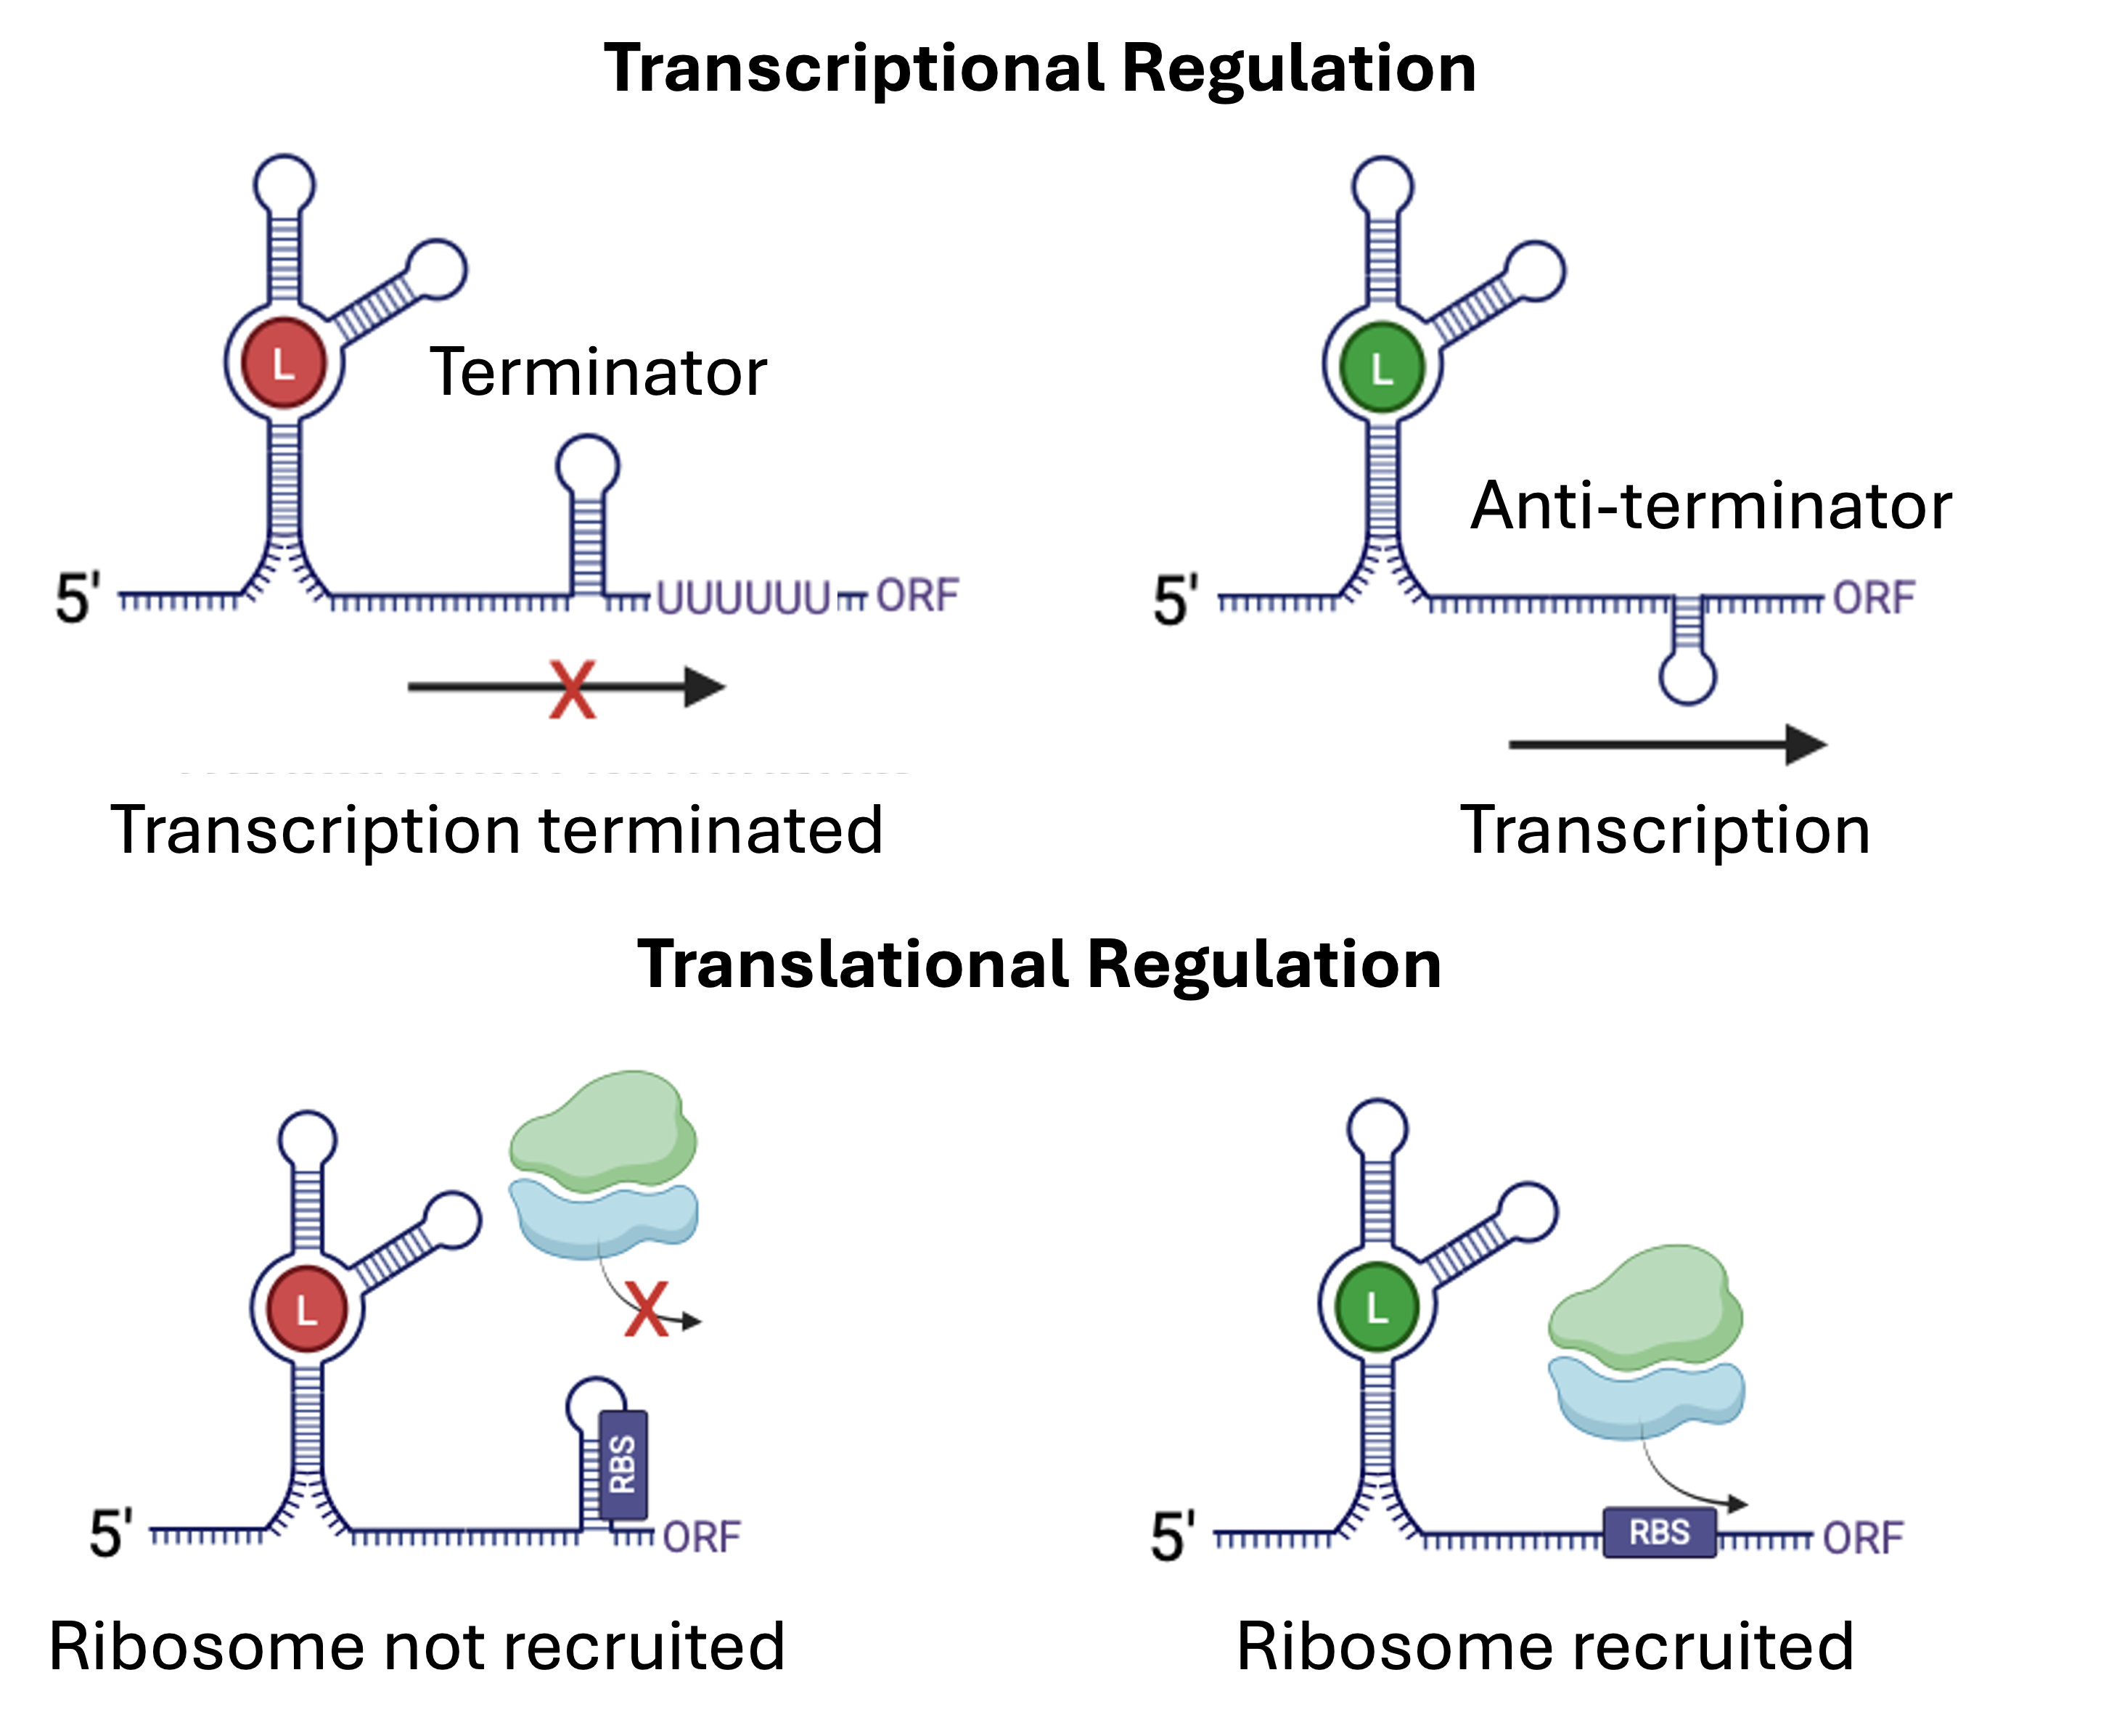
\includegraphics[width=0.8\textwidth]{figures/riboswitch-mechanism.png}
    \caption{\textbf{Typical riboswitch regulatory mechanisms.} 
    Riboswitches control gene expression through ligand-induced conformational changes that affect either transcription or translation.
    Ligands ("L") bind aptamers resulting in 
    \textbf{Transcriptional control (top):} Riboswitches can either promote an early termination when ligand-bound (left) or prevent termination (right) allowing transcription through the ORF. 
    \textbf{Translational control (bottom):} Riboswitches can either make the ribosome binding site less accessible (left) or more accessible (right) when ligand-bound.
    ORF = open reading frame; RBS = ribosome binding site. 
    Created in  https://BioRender.com}
    \label{fig:riboswitch-mechanism}
\end{figure}

Transcriptional riboswitches control formation of Rho-independent terminators—intrinsic termination structures consisting of a hairpin followed by a uridine-rich tract. 
Depending on the riboswitch, ligand binding may promote terminator formation or stabilize an antiterminator structure, enabling transcriptional read-through.
Similarly, translational riboswitches can sequester or expose the ribosome-binding site in response to ligand binding \parencite{Breaker2023}.

\subsubsection*{Biotechnological Applications}

RNA has been central to several majoy biotechnological breakthroughs. 
CRISPR-Cas9 gene editing harnesses guide RNAs for programmable genome modification \parencite{Jinek2012}. 
mRNA vaccines against COVID-19 demonstrated the therapeutic potential of synthetic mRNAs \parencite{Polack2020}. 
RNA interference (RNAi) enables targeted gene silencing in research and therapeutics \parencite{Fire1998}.

RNA aptamers such as Spinach bind fluorogenic compounds and fluoresce upon binding, enabling RNA visualization in living cells \parencite{Paige2011}.
The photoriboswitch Werewolf-1, generated through \emph{in vitro} selection, responds to light by binding photoisomerizable ligands, offering potential for optogenetic control of gene expression \parencite{Rotstan2020}.
These RNAs, involved in fluorescence and photoreception, have broad relevance for medical research, biotechnology, and agricultural applications \parencite{Micura2020}.

\subsection{Current Approaches to Functional RNA Discovery}

It is predicted that a large number of riboswitches remain undiscovered, potentially on the order of thousands \parencite{Kavita2023}.
Ronald Breaker and colleagues have pioneered systematic riboswitch and ribozyme discovery, identifying over 55 distinct riboswitch classes to date \parencite{Breaker2022}.
Other major RNA-related discoveries, such as ribosomes and CRISPR-Cas systems, occurred through more exploratory research approaches \parencite{Brück2025}.

\subsubsection*{Experimental Approaches}

Transcriptome mapping approaches have proven successful for unbiased riboswitch discovery. 
Term-seq maps RNA 3' termini genome-wide to identify premature transcription termination sites characteristic of riboswitches and attenuators \parencite{Dar2016}. This approach discovered numerous antibiotic-responsive riboswitches controlling resistance genes in bacterial pathogens and the human microbiome. 
This approach has uncovered numerous antibiotic-responsive riboswitches controlling resistance genes in bacterial pathogens and within the human microbiome.
RNA structure probing methods characterize secondary structures, tertiary interactions, and dynamic conformational changes. 
SHAPE-seq (Selective 2'-Hydroxyl Acylation analysed by Primer Extension Sequencing) chemically modifies unpaired nucleotides, enabling genome-wide structure mapping \parencite{Lucks2011}. 
This approach can identify structured regions throughout transcriptomes, revealing RNA switches, ribozymes, and protein-binding sites.
DMS-MaPseq extends this approach to structural probing \emph{in vivo} \parencite{Zubradt2017}.
A variety of methods exist for studying protein-RNA interactions from both protein- and RNA-centric approaches \parencite{Yi2025}.

While powerful for validation and mechanistic characterization, experimental approaches are labour-intensive, may miss RNAs with unknown functions, and are difficult to scale across many organisms.

\subsubsection*{\emph{In Vitro} Selection and Computational Design}

\emph{In vitro} selection (SELEX) generates novel functional RNAs by applying selective pressure to a library of random sequences.
This technique was used in the generation of the photoriboswitch, Werewolf-1 \parencite{Rotstan2020}.
Generation of synthetic functional RNAs by computational design has also been reported, with tools like RfamGen and RhoDesign \parencite{Sumi2024}.

Many RNA discoveries, including CRISPR-Cas systems, mRNA vaccine strategies and many catalytic RNAs were however discovered in nature, not designed \emph{de novo} \parencite{Micura2020,Barrangou2007}.
Beyond biotechnology, fundamental understanding of natural RNA-based systems has value, for example the discovery of flouride sensing riboswitches in bacteria \parencite{}

\subsubsection*{Computational Approaches}

Bioinformatic sequence-based searches using tools like BLAST identify homologous sequences, but many functional RNAs have divergent sequences detectable only through structural conservation.
Structure based searches have proven successful, like the bioinformatic search for twister ribozymes by \textcite{Roth2014} discovering roughly 2,700 ribozymes.
These techniques search on sequence and secondary structure patterns, but require existing alignments and structure models, limiting their utility for discovering entirely novel RNA classes.

RNA structure prediction remains a challenging problem, particularly when given a single sequence and no homology structures are known, as would be the case with a genome wide search for novel RNA structures in a single species.
Comparative approaches using multiple homologous sequences provide greater predictive power for RNA structure inference \parencite{Kagaya2026}.

Comparative genomics leverages evolutionary conservation of RNA structures across related species, enabling the identification of conserved structural features.
These conserved features are termed RNA motifs, regions showing evidence of selective constraint on structure, indicating potential functional importance. 
Such motifs may represent riboswitches, ribozymes, or other classes of functional RNAs.

Zasha Weinberg's lab has had notable successes with their tool CMfinder, \textcite{Yao2006}, which identifies conserved RNA secondary structures using a comparative genomics approach.
The \textcite{Sack2025} paper, also from the Weinberg lab, recently identified 16 new structured RNA classes in plants using a CMfinder-based bioinformatic screen.
This study focused on structured RNAs involved in alternative splicing.

\textcite{Roth2014} also employed CMfinder to identify a new class of self cleaving ribozymes, the twister ribozyme, which has since been found to be widespread in nature.
In that paper hammerhead and twister ribozymes were observed to commonly reside near each other and to certain protein coding genes, although noting it still a biological mystery. 
\textcite{Weinberg2015} followed up on this observation with a screening of sequences nearby known ribozyme and ribozyme associated protein domain coding regions.
This approach successfully identified additional ribozyme classes including pistol and hatchet.

\subsection{Gene Family-Targeted Searches}

Beyond the successes of gene family-targeted searches with CMfinder, there is precedent for riboswitches being encoded upstream of certain gene families \parencite{Micura2020, Kavita2023}.
This approach also provides a less computationally intensive alternative to genome-wide screens, allowing for wider searches across more species.
Harnessing the power of evolutionary conservation and leveraging the biological assumption that functionally related genes (i.e. with domain homology) may share regulatory mechanisms.

Due to its potential importance in biotechnology this project will be screening for conserved RNA structures located near light-sensing gene families.
Light-sensing systems in bacteria often involve complex regulatory networks, and RNA-based mechanisms have been shown to play roles in light acclimation responses in cyanobacteria \parencite{Hihara2015}.

A recent study by a group in Copenhagen, \textcite{Geissler2026}, describes a bioinformatic screen similar to the one undertaken here.
In that work orthologous cyanobacteria genes involved in photosynthetic pathways were targeted for nearby conserved RNA structure discovery using CMfinder.
Approximately 400 novel conserved RNA structures were identified.

\subsection{Bacterial Genomes as a Search Space}

Riboswitches have been most extensively discovered and experimentally validated in bacteria and seem to rarely have homologs in eukaryotes \parencite{Kavita2023}.
This makes bacteria a reasonable domain for riboswitch discovery efforts.

Extensive phylogenetic diversity is available among sequenced bacterial genomes.
As of April 2026, over 870,000 bacterial genomes spanning 180,000 bacterial species clusters have been sequenced and organised in databases such as the Genome Taxonomy Database \parencite{GTDB2026}.
This represents vast evolutionary distances, bacteria diverged over 3 billion years ago, providing the deep phylogenies necessary for detecting conserved structures through covariation analysis.

Bacterial regulatory mechanisms are generally simpler than eukaryotic systems, with less complex post-transcriptional processing and more direct coupling between transcription and translation. 
This simplifies both computational predictions and experimental validation.

% Project aims (should be about half a page)
\subsection{Aims}

The overarching aim is to discover novel functional RNA motifs associated with bacterial light-sensing systems by leveraging comparative genomics. 
Gene-family-targeted approaches offer a computationally tractable approach for identifying regulatory elements linked to specific biological pathways. 
Light-sensing gene families are of particular interest due to their importance in environmental adaptation and their potential relevance to biotechnological applications. 
Identifying conserved RNA structures associated with these genes may reveal previously uncharacterized regulatory mechanisms.

The first aim of this project is therefore to identify evolutionarily conserved RNA structural motifs located near light-sensing gene families across diverse bacterial lineages. 
By examining intergenic and transcript regions associated with these genes, the project aims to predict conserved RNA secondary structures using comparative genomics approaches that identify covariation patterns indicative of selective constraint.
These may represent riboswitches, ribozymes, or other regulatory elements. 

The second aim is to develop a generalizable comparative genomics pipeline using modern tools, capable of systematically screening for conserved RNA structures linked to specific protein domain families. 
This pipeline is intended to be reusable and adaptable for future studies, targeting additional gene families or biological pathways. 

Together, these aims will contribute both new candidate RNA motifs and a methodological platform for search for structured RNAs in nature.

\subsection{Hypothesis}

Evolutionarily conserved structural motifs within transcripts associated with specific gene families represent functional regulatory elements maintained by natural selection.
These elements may employ diverse mechanisms, including ligand-dependent structural switching (riboswitches), catalytic self-cleavage (ribozymes), protein binding, or other structure-based regulatory strategies, to control gene expression.

% Bibliography
\newpage
\printbibliography

\end{document}


\chapter{Methods}

An overview of the approach used in this study is provided in Figure \ref{fig:methodsoverview}.
The main computational discovery pipeline uses data curated from public datasets to search for conserved structured RNA elements encoded near a conserved protein domain anchor.
Conversely, the positive control pipeline searches for conserved protein domains starting from a known RNA element anchor, acting to validate both the discovery pipeline and the premise of this project.

In addition to the main discovery and positive control pipelines, iterative expansion and covariance model clustering approaches are described as downstream analyses for identified candidates.

\begin{figure}[H]
    \centering
    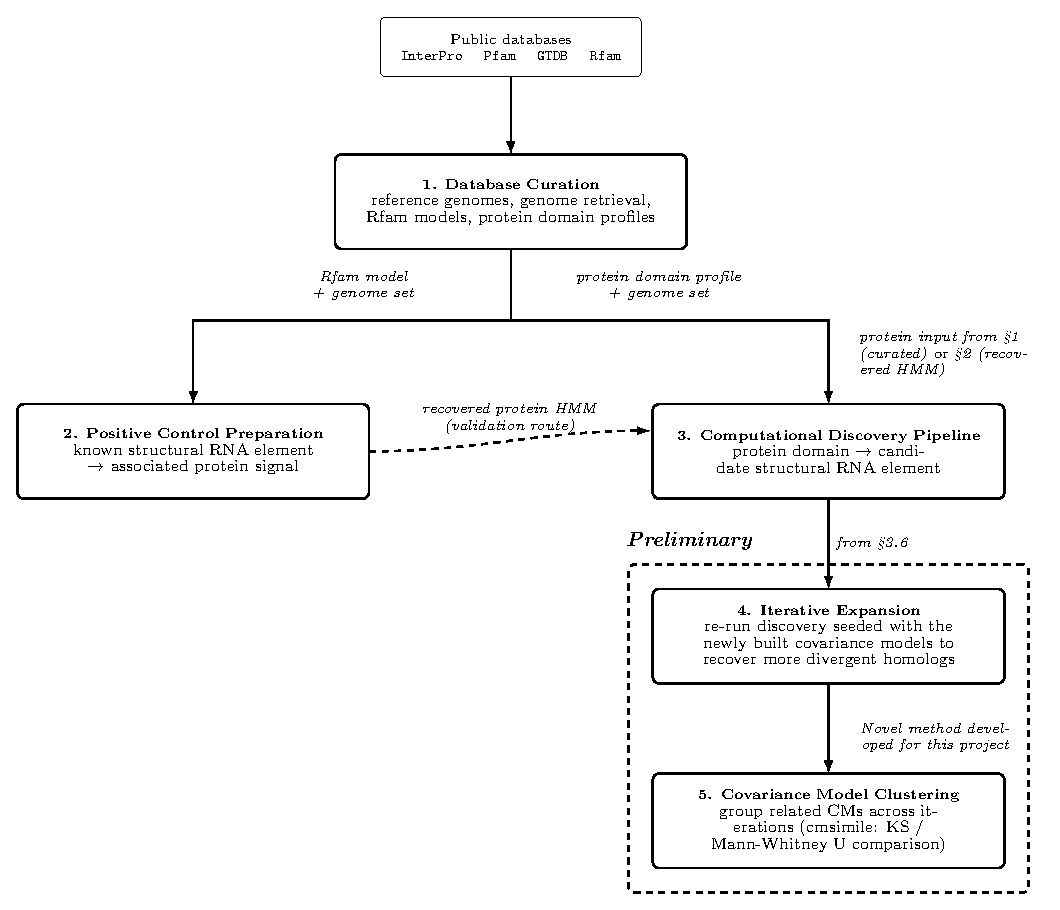
\includegraphics[width=0.95\textwidth]{figures/methods/overview.pdf}
    \caption[Overview of methods]{\textbf{Overview of methods}
    Simplified overview of the approach taken for \ac{RNP} candidate discovery. Numbered steps refer to the following subsections. }
    \label{fig:methodsoverview}
\end{figure}

The discovery and positive control pipelines are written in Python 3.14.6 using Snakemake v.9.23.1, and are configurable and automated \citep{Molder2025}.
Iterative expansion and covariance model clustering were developed in Go v.1.27.1 and are available as standalone tools.
All code, software environment definitions and data used in this study are available in the supplementary materials (Appendix \ref{sec:code-and-data-availability}).

\section{Database curation}

% abstract steps from discovery and positive control pipeline, and describe the databases used and versions.

% \begin{figure}[H]
%     \centering
%     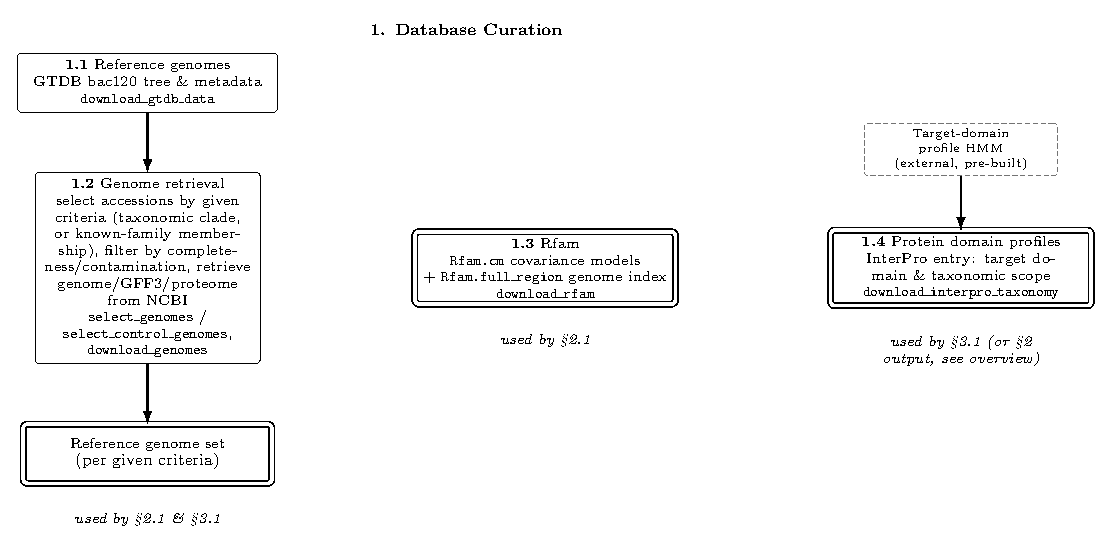
\includegraphics[width=0.95\textwidth]{figures/methods/section1_database_curation.pdf}
%     \caption[Database curation]{\textbf{Database curation}
%     An overview of the databases used and filtering and curation steps taken. 
%     Numbered steps refer to the subsections below. 
%     In bold are custom script and assets retrieved from online public databases.}
%     \label{fig:databasecuration}
% \end{figure}



\subsection{Reference genomes}
\label{subsec:reference-genomes}

For all analyses, the \ac{GTDB} release 232 \citep{Parks2022} was used to select a diverse set of bacterial genomes for analysis. 
The GTDB provides a standardised taxonomy, ensuring that the selected genomes are representative of the bacterial domain. 
Python package ete3 v.3.1.3 \citep{huertacepas2016} was used for phylogenetic analysis and filtering using the \ac{GTDB} phylogenetic tree.
Further filtering was performed to select high-quality, complete genomes (completeness $>$ 99.9\%, contamination $<$ 1\%), ensuring the selected reference genomes are suitable for downstream analysis.
Completeness and contamination metrics were provided by CheckM2 \citep{Chklovski2023}, available in the \ac{GTDB} release.

\subsubsection{Genome retrieval}
\label{sec:genomes}

Only genomes with genomic sequence, protein sequence and annotation files available were retrieved from the \ac{NCBI} GenBank database release 265.0 \citep{OLeary2024}.

Full lists of genomes used in this study for particular experiments are available in the supplementary materials (Appendix \ref{sec:code-and-data-availability}).

\subsection{Covariance models}
\label{subsec:covariance-models}

RNA family covariance models were retrieved from the Rfam database (version 15.0) \citep{Ontiveros-Palacios2025}.
These were used in positive control experiments to validate the pipeline and to identify known RNA families among the candidates identified.

Additionally, covariance models and clan information available from the Rfam database (version 15.0) \citep{Ontiveros-Palacios2025} were used to validate the clustering method developed in this study.
Seed sequences (curated members of each family, used to build the alignments from which the family models are built) were also retrieved.

\subsection{Protein domain profiles}
\label{subsec:protein-hmm-retrieval}

InterPro (version 35.0) entries guided the choice of protein domain model and relevant genome search space \citep{Blum2025}.
Protein domain \ac{HMM} profiles were retrieved from the Pfam v.35.0 database \citep{Paysan-Fafosse2025}.
These were used in the discovery pipeline to search for protein homology to anchor the search for conserved structured RNA elements.

% -------- rna -> protein ------------

\section{Positive control preparation}
\label{sec:poscontrol-pipeline}


\begin{figure}[htbp]
    \centering
    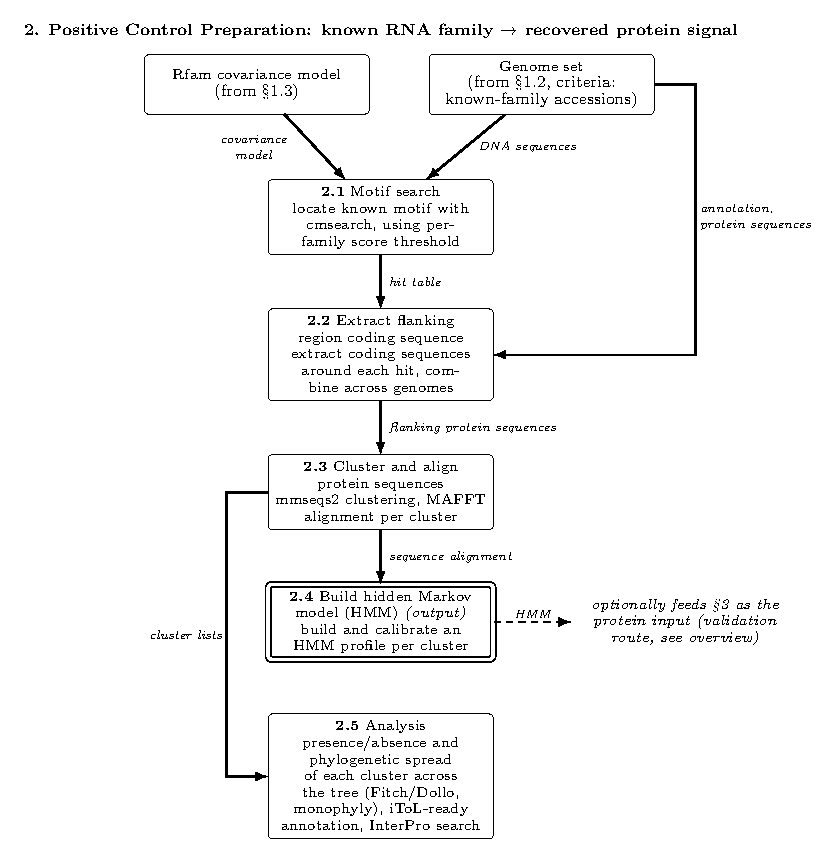
\includegraphics[width=0.95\textwidth]{figures/methods/section2_positive_control.pdf}
    \caption[Positive control preparation] {\textbf{Positive control preparation (known RNA family $\rightarrow$ recovered protein signal).}
    Starting from Rfam covariance models (\S\ref{subsec:covariance-models}) and genomes containing known family members (\S\ref{sec:genomes}), the pipeline locates each known element with cmsearch, extracts
    the flanking coding sequences, and clusters and aligns the encoded proteins. 
    Coding sequences within 1000\,nt of each hit were extracted. 
    Proteins were clustered with MMseqs2 (sensitivity 7.5, minimum sequence identity 0.25, coverage $\geq 0.2$), and clusters with fewer than 5 members were discarded.
    Italic labels show the data passed between steps. A hidden Markov model is built and calibrated for each cluster (double border, output) and can optionally feed the discovery pipeline as the protein input. 
    Clusters are also analysed for presence/absence and phylogenetic spread across the tree, and searched against InterPro.
    Hits were called using the Rfam per-family score thresholds and covariance models.}
    \label{fig:poscontrol}
\end{figure}

Pipeline inputs are Rfam covariance models and annotated seed sequences, as described in Section~\ref{subsec:covariance-models}.
A custom script accessing Entrez via the Python Biopython v.1.87 library searches for genomes containing these sequences \citep{OLeary2024}.
A genome set is then constructed from \ac{GTDB} reference genomes and downloaded from GenBank (Section~\ref{subsec:reference-genomes}).
All inputs from runs of this pipeline used in this study are available in Table \ref{tab:positive_controls_input}.

\subsection{RNA structure search}

Members of the Rfam family were searched using the Rfam published search parameters, to revalidate hits and confirm coordinate system in reference genomes (Infernal v.1.1.5 \emph{cmsearch}).
The output of this step is a list of genomic coordinates for each hit, which is used to extract the flanking coding sequences.

\subsection{Extract flanking coding sequences}

Coding sequences surrounding the RNA element locus are extracted from the genome, within a 1000 nucleotide region.
This was done to identify protein domains that are encoded in close proximity to the RNA element, which may indicate a functional relationship between the two.
The approach is illustrated in Figure \ref{fig:flankingcds}.

\begin{figure}[H]
    \centering
    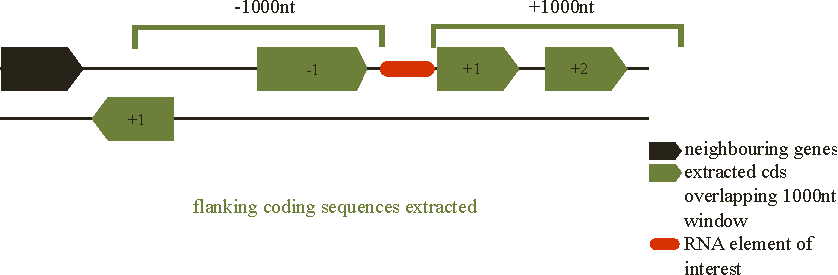
\includegraphics[width=0.8\textwidth]{figures/methods/flanking_cds_fig.pdf}
    \caption[Flanking coding sequence extraction]{\textbf{Flanking coding sequence extraction.}
    Annotated coding sequences surrounding the RNA element of interest are extracted from genomes within a 1000 nucleotide region.
    Shown in red is the RNA element of interest identified by cmsearch, in black is a coding sequence outside the 1000 nucleotide extraction region.
    Indicated in green are the flanking coding sequences extracted for further analysis, labelled by upstream (+) or downstream (-) of the RNA element as well as the order (1 or 2 upstream or downstream). 
    Strandedness of the surrounding coding sequences is also recorded (same or different to the cmsearch hit).}
    \label{fig:flankingcds}
\end{figure}

Reference genome annotation files were used to identify the coding sequences flanking the RNA element of interest, using coordinates from the RNA structure search output by a custom script.
Protein sequences of these identified coding sequences were then extracted from the genome and used for downstream clustering and alignment.

\subsection{Clustering and aligning protein sequences}

\subsubsection{Clustering}

Protein homology was assessed by clustering the extracted protein sequences.
Protein sequences were clustered using MMseqs2 v.14.7.0 \citep{Steinegger2017}.
The clustering was performed with a sensitivity of 7.5, a minimum sequence identity of 0.25, and a minimum coverage of 0.2.
Clusters with fewer than 5 members were discarded to ensure that only clusters with sufficient representation were retained for further analysis.

\subsubsection{Sequence alignment}

A \ac{MSA} was built using from the trimmed cluster sequences (MAFFT v.7.525) \citep{Katoh2013}.
This identifies conserved sequence features and provides a basis for secondary structure prediction and covariance model building.
Alignments also describe how sequences are related to each other, which is important for downstream analyses such as covariance model building and iterative expansion.


\subsection{Build \ac{HMM}}
\label{sec:positive_control_hmm}

Probabalistic models, \ac{HMM}s, were built based on the \ac{MSA} of each alignment.
This was done to capture the sequence diversity of each cluster, and to allow for sensitive searches for homologous sequences in the discovery pipeline.
HMMER v.3.4 \emph{hmmbuild} and \emph{hmmcalibrate} were used to build and calibrate the \ac{HMM}s.

\subsection{Analysis}

The pipeline reports the results of the computational analysis, the prevelence of cluster members across the reference genomes.
The position of the protein domain relative to the RNA element is also reported, as well as the number of clusters identified and their sizes.

\subsubsection{Taxonomic spread analyses with \ac{iTOL}}

Monophylicity or polyphylicity of clusters was assessed by mapping the presence or absence of cluster members to the \ac{GTDB} phylogenetic tree.

An annotation file was generated for each cluster, indicating the presence or absence of a cluster member in each genome.
This was visualised on the \ac{iTOL} v.7 online tool \citep{Letunic2024} to assess the taxonomic spread of each cluster, and identify bacterial clades where the cluster is more abundant for positive control inputs of the discovery pipeline.

\subsubsection{Identification with InterPro}

Cluster sequences were submitted to the online InterProScan v.6 tool; the results indicated the protein hits and what the protein signal represents \citep{Blum2026}.
Pfam v.35.0 entries were reported for the highest prevalence cluster, and the InterPro entry was used to identify the protein domain represented by the cluster.

% -------- protein -> rna ------------

\section{Computational discovery pipeline}
\label{sec:computational-discovery-pipeline}

\begin{figure}[htbp]
    \centering
    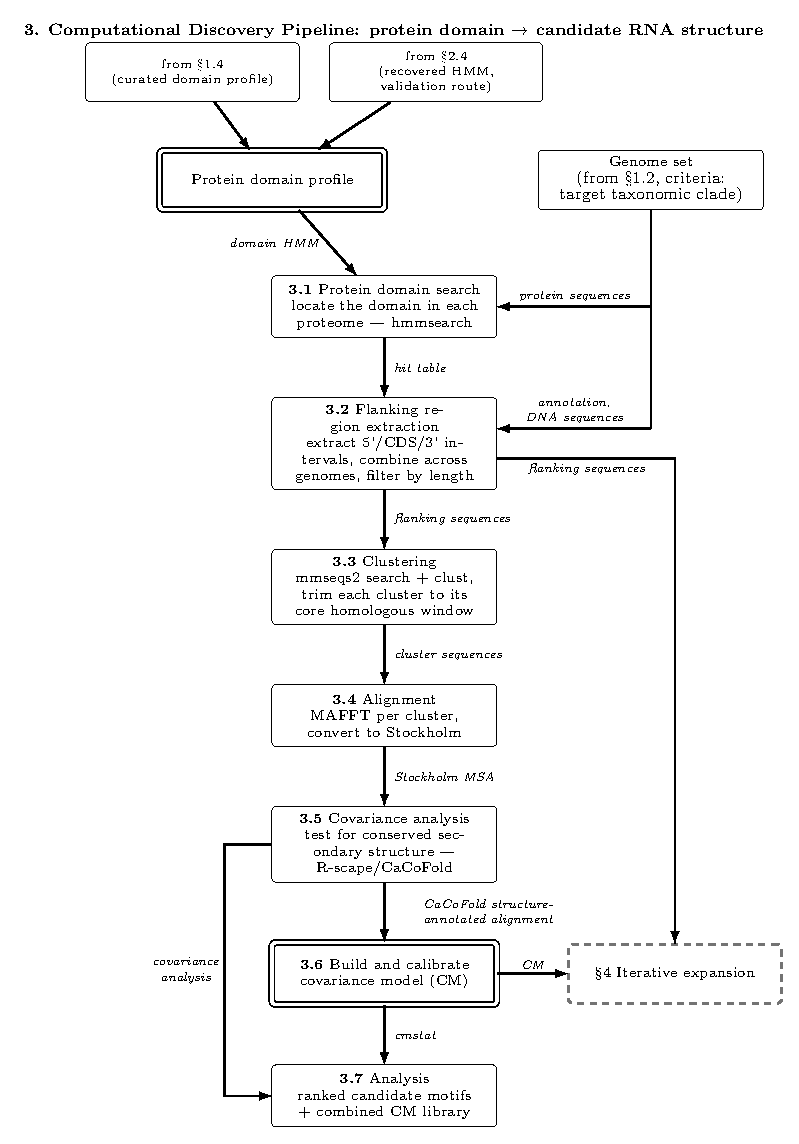
\includegraphics[width=0.95\textwidth, height=0.72\textheight, keepaspectratio]{figures/methods/section3_discovery_pipeline.pdf}
    \caption[Computational discovery pipeline]{%
    \textbf{Computational discovery pipeline (protein domain $\rightarrow$ candidate structured RNA).}
    A protein domain profile, either curated (\S\ref{subsec:protein-hmm-retrieval}) or recovered from the
    positive control (\S\ref{sec:positive_control_hmm}), is searched against the proteomes of the
    target clade (\S\ref{subsec:reference-genomes}). Flanking regions of each hit are extracted, clustered,
    aligned and tested for conserved secondary structure, and covariance models are built from
    the structure-annotated alignments (double border, output). Candidate structured RNAs are
    ranked in the final report, and the covariance models and flanking sequences pass to
    iterative expansion (\S\ref{sec:iterative}). Italic labels show the data passed between
    steps. Filtering thresholds are given in Table~\ref{tab:thresholds}.}
    \label{fig:discovery}
\end{figure}


Inputs of the pipeline are a protein domain \ac{HMM} which serves as an anchor for the search, sourced as described in Section~\ref{subsec:protein-hmm-retrieval}, and a selection of reference genomes as a search space (Section~\ref{subsec:reference-genomes}).
For validation the protein domain \ac{HMM} is one recovered from the positive control pipeline (Section~\ref{sec:poscontrol-pipeline}).
All inputs from runs of this pipeline used in this study are available in Table \ref{tab:discovery_inputs}.

\subsection{Protein domain search}

Protein homology was searched using a probabilistic model (\ac{HMM}) against the genome sequence set (Section~\ref{subsec:reference-genomes}) (\emph{nhmmer} hmmer v3.4).
To narrow the search for structured RNAs, the search was focused to regions flanking the identified protein domains.

\subsection{Flanking region extraction}
\label{sec:flanking}

% describe approach, and filtering done
The flanking regions are extracted from the reference genomes' genomic sequence based on the coordinates of the protein domain hits and the genomic annotations.
The extracted sequences are then filtered for length and quality to ensure that only high-quality sequences are used in subsequent steps.
Figure~\ref{fig:flankingregion} illustrates the flanking region extraction process, where the anchor coding sequence is identified by \emph{nhmmer}, and the annotated up and downstream coding sequences of the same strand are used to define the flanking regions.

\begin{figure}[H]
    \centering
    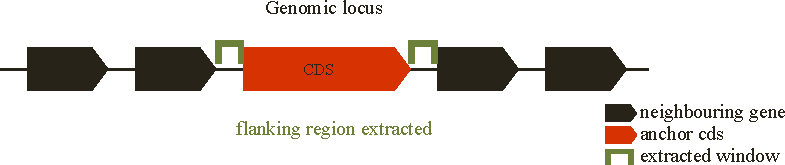
\includegraphics[width=0.8\textwidth]{figures/methods/extracted_flanks.pdf}
    \caption[Flanking region extraction]{\textbf{Flanking region extraction.}
    Non-coding flanking DNA sequence is extracted from genomes based on hmmer hits in protein sequence and published genome annotations.
    Shown in red is the anchor coding sequence identified by nhmmer, in black are annotated up and downstream coding sequences of the same strand.
    Indicated in green are the flanking regions extracted for further analysis. }
    \label{fig:flankingregion}
\end{figure}

Length filtering included only sequences $\geq 20$ nucleotides to allow for meaningful homology searches in subsequent clustering steps.

\subsection{Sequence clustering}

\subsubsection{MMseqs2 clustering}
\label{subsec:clustering}

Flanking sequences were clustered with a pairwise search based on sequence similarity with MMseqs2 v.16.747c6 \emph{search} \citep{Kallenborn2025}.
This was done to group sequences that are likely to be homologous, and to reduce the number of sequences for downstream analyses.

\subsubsection{Sequence trimming}

Clustered sequences are then trimmed to the local-alignment window it shares (directly or transitively) with an anchor sequence from the same cluster, using coordinates from a single all-vs-all search pass (MMseqs2 v.16.747c6).
Window lengths were filtered to include those of length $\geq 15$ and $\leq 1000$ nucleotides.
A padding of 15 nucleotides was kept on either side of this window.
These trimming and filtering steps were implemented to remove spurious flanking sequence and to focus on the conserved region of the cluster.

\subsection{Sequence alignment}
\label{subsec:rna-alignment}

A \ac{MSA} was built using from the trimmed cluster sequences (MAFFT v.7.525) \citep{Katoh2013}.
This identifies conserved sequence features and provides a basis for secondary structure prediction and covariance model building.
Alignments also describe how sequences are related to each other, which is important for downstream analyses such as covariance model building and iterative expansion.

\subsection{Covariance analysis}
\label{subsec:covariance-analysis}

The CaCoFold algorithm of R-scape v.2.0.4 was used to predict conserved secondary structure and covarying base pairs in the \ac{MSA} \citep{Rivas2017}.
This approach tests for covariation in the alignment, and predicts a consensus structure based on the covarying base pairs.
It provides a structure-annotated \ac{MSA} in Stockholm format, which can be used to build a covariance model.
Additionally, it provides a statistical test for covariation, giving an $E$-value for each predicted covarying base pair, statistical power for the covariation test, and an F-value for the overall alignment (the harmonic mean of sensitivity (SEN) and positive predictive value (PPV)).
Secondary structure diagrams were generated with R2R v.1.0.6 \citep{Weinberg2011}.

This covariance analysis step is the key step in the pipeline to identify any structured RNA elements.
$E$-values for covarying base pairs are used to filter out spurious predictions, and the overall F-value is used to assess the quality of the alignment.

\subsection{Covariance model construction and calibration}
\label{sec:build_cm}

Filtering was done on the CaCoFold structurally annotated alignments to include only those with at least one covarying pair where $E \le 0.05$.
The Infernal v.1.1.5 \emph{cmbuild} tool was used to generate probabilistic models from identified CaCoFold generated structural alignments, default parameters were used.
Infernal v.1.1.5 \emph{cmcalibrate} assigns $E$-values to built models by fitting exponential tails to the hits of random sequences, this is required for statistical significance in searches using these models \citep{Nawrocki2013}.
\acp{CM}s with calibration runtimes $< 3$ hours and requiring $< 8$ \ac{Gb} space on 4 \ac{CPU} cores were calibrated with \texttt{-{}-tailp 0.05}, fitting the null tail from the top 5\% of the histogram.
The random sequence set size was also limited in size to 0.8 \ac{Mb}, this trades off $E$-value accuracy for quicker run times.

\subsection{Analysis}

Most analysis of the discovery pipeline is done by validation with the positive control pipeline, and by downstream by iterative expansion of the covariance models (Section~\ref{sec:iterative}).
Addititionally negative control protein domains were used to assess the behaviour of the discovery pipeline when applied to protein domains that are unlikely to be associated with structured RNA elements.
The parameters of the clustering step were adjusted with the positive control run to find a balance between sensitivity and specificity, and to cluster size (Appendix Figure~\ref{fig:poscontrol-clustering}).

% ------- cm-iterative-expansion -----

\section{Iterative expansion}
\label{sec:iterative}

% explain the idea that starting from 
The idea of this iterative expansion approach is to use the probabilistic models (covariance models) built by the discovery pipeline to search for further homologous sequences in the flanking sequence set.
This was done by an iterative approach described in Figure~\ref{fig:iterative-expansion} using the Infernal v.1.1.5 toolkit \citep{Nawrocki2013}.
The probabilistic models describe sequence and structural information, and as such can be used to search for likely homologs.
These models can be used to align those homologs, and new models can be built from the resulting alignments.

\begin{figure}[H]
    \centering
    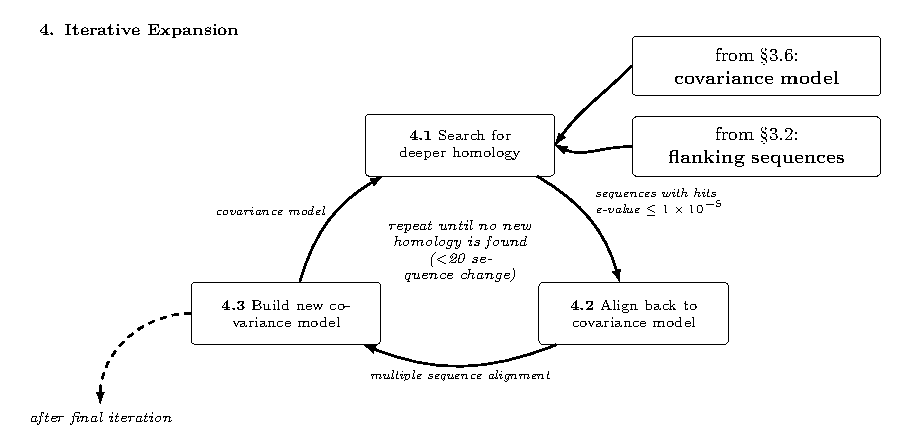
\includegraphics[width=0.95\textwidth]{figures/methods/section4_iterative_expansion.pdf}
    \caption[Iterative expansion of candidate covariance models]{%
    \textbf{Iterative expansion of candidate covariance models.}
    Each covariance model from \S\ref{sec:build_cm} is used to search the flanking sequences from \S\ref{sec:flanking} for deeper homology (4.1) with Infernal v1.1.5. 
    Sequences with hits at an $E$-value $\leq 1\times10^{-5}$ are aligned back to the covariance model (4.2), and a new covariance model is built from the resulting multiple sequence alignment (4.3). 
    The cycle repeats until $<$20 new homologous sequences are found. 
    The dashed arrow marks exit from the loop after the final iteration.}
    \label{fig:iterative-expansion}
\end{figure}

For all uses of this iterative expansion pipeline, a convergence cut-off of 20 new sequences identified in a round was used.
This was to avoid long or infinite iterations.
When this convergence limit was met a final covariance model and alignment was returned as output.

\subsection{Search for deeper homology}

The probabilistic models (covariance models) built by the discovery pipeline were used to search for further homologous sequences in the flanking sequence set (Infernal v.1.1.5 \emph{cmsearch}).
An $E$-value threshold of $1\times 10^{-5}$ was applied to retain significant hits, with otherwise default parameters.
Resulting identified sequences were aligned back to the covariance model.

\subsection{Align back to covariance model}

Infernal v.1.1.5 \emph{cmalign} was used to align identified homologous sequences back to the covariance model of interest \citep{Nawrocki2013}.
This produces a structure-annotated \ac{MSA} of the identified sequences, which can be used to build a new covariance model, potentally adding new structural and sequence information.
These alignments were generated with default parameters as structure-annotated, Stockholm-formatted \acp{MSA}.

\subsection{Build new covariance model}

Probabilistic models describing the structure and sequence of the RNA homology identified in the previous steps were built.
Infernal v.1.1.5 \emph{cmbuild} and \emph{cmcalibrate} were used to build and calibrate new models from the expanded \acp{MSA} \citep{Nawrocki2013}.
Structure was preserved between rounds with the \emph{cmbuild} \texttt{-{}-hand} option, and default \emph{cmcalibrate} parameters.

\subsection{Analysis}

The iterative expansion pipeline outputs are structure-annotated, Stockholm-formatted \acp{MSA}s and calibrated covariance models.
Reported also are the number of rounds of expansion, and the number of sequences identified in each round.
Analysis of the output covariance models was done with the covariance model clustering pipeline (Section~\ref{sec:cm-simile}).
\ac{MSA}s resulting from positive control candidates of the discovery pipeline were also analysed for hit identity and coverage.
Hit identity was calculated as the number of identical sequences between alignments.
Coverage identity was calculated using the coordinates of the alignment sequences, as the number of identical nucleotides between alignments divided by the total length of all alignment sequences.
This was calculated as the intersection / union of the alignment coordinates.
All analysis was done with custom R v.4.6.1 scripts, and plotted with ggplot2, available in the supplementary materials (Appendix~\ref{sec:code-and-data-availability}) \citep{Wickham2016}.

% -------- cm-simile ------------

\section{Covariance model clustering}

An overview of the approaches taken to quantify relatedness between covariance models is provided in Figure~\ref{fig:cm-similarity-approaches}.
These approaches were developed to quantify relatedness between covariance models, and to cluster them based on this relatedness.
This is described in more detail in the following subsections.

\begin{figure}[htbp]
    \centering
    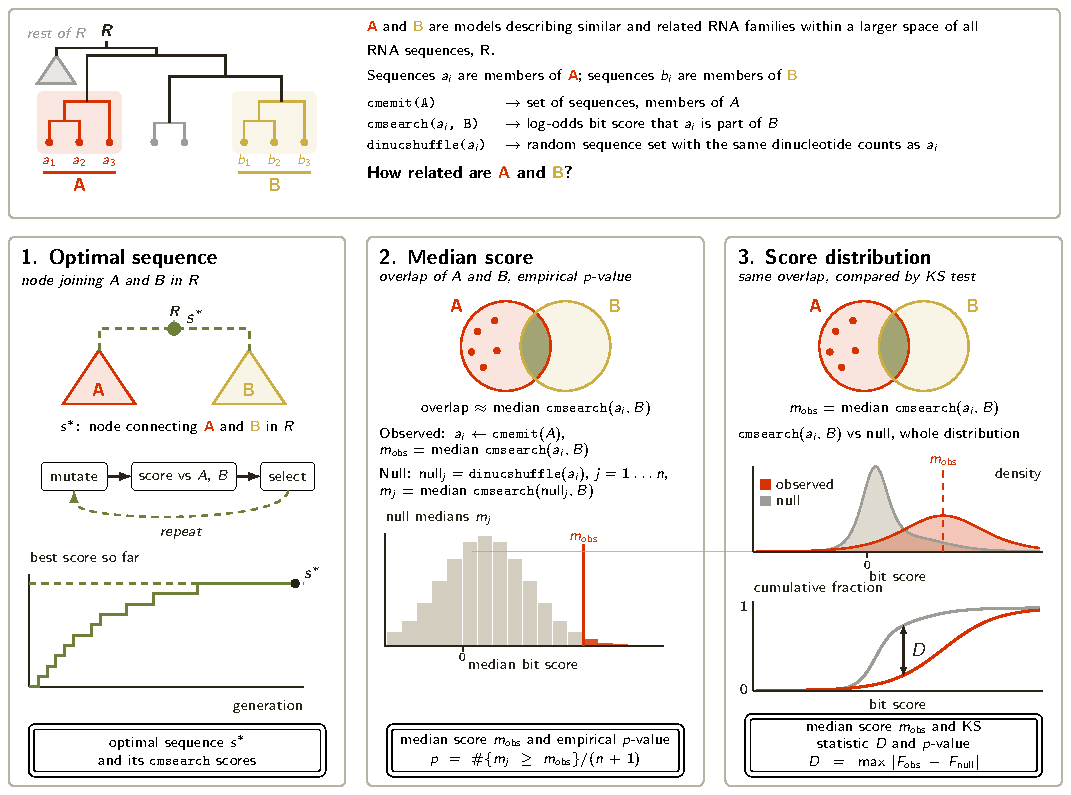
\includegraphics[width=1\textwidth]{figures/methods/section5_cmsimile_approaches.pdf}
    \caption[Approaches for quantifying relatedness between covariance models]{%
    \textbf{Three approaches for quantifying how related two covariance models are.}
    Models $A$ and $B$ describe related RNA families within the space of all RNA sequences, $R$; sequences $a_i$ are members of $A$ and $b_i$ are members of $B$. 
    Sequences are sampled from a model with \emph{cmemit}, scored against a model with \emph{cmsearch} (log-odds bit score), and null sequences are generated by dinucleotide shuffling.
    \textbf{(1) Optimal sequence:} an evolutionary search mutates candidate sequences, scores them against both $A$ and $B$, and selects the best, repeating over generations to approximate the sequence $s^{*}$ that joins the two families; the scores of $s^{*}$ against each model are reported.
    \textbf{(2) Median score:} the median bit score of sequences emitted from $A$ and searched against $B$ ($m_{obs}$) is compared with the medians of $n$ bootstrap resamples of the pooled scores of dinucleotide-shuffled sequences ($m_j$), giving an empirical $p$-value, $p = (1 + \#\{m_j \geq m_{obs}\})/(n + 1)$.
    \textbf{(3) Score distribution:} the full distribution of bit scores is compared with the null using a two-sample Kolmogorov--Smirnov test, where the statistic $D$ is the maximum difference between the observed and null cumulative distributions.}
    \label{fig:cm-similarity-approaches}
\end{figure}

\subsection{Sequence scoring}
\label{sec:sequence-scoring}

Sequences were scored against each model with the Infernal v.1.1.5 tool \emph{cmsearch}, giving a log-odds bit score for each sequence against each model.

\begin{equation} 
S_{\mathrm{bit}}(x)
=
\log_2
\left[
\frac{P(x \mid A)}
     {P(x \mid \varnothing)}
\right]
\end{equation}

where $x$ is a sequence, $A$ is a covariance model, and $\varnothing$ is the null model of random sequence.

\subsection{Sequence sampling}
\label{sec:sequence-sampling}

Sequences were sampled from each probabilistic model (covariance model) with the Infernal v.1.1.5 tool \emph{cmemit}.

\subsection{Null sequence pool generation}
\label{sec:dinuc-shuffle}

Null sequences were generated by an implementation of the Dinucleotide Shuffle algorithm first described by \citet{Altschul1985}.
This approach preserves 2-mer composition while destroying any underlying structure or sequence conservation.

\subsection{Pairwise similarity scoring approaches}

\subsubsection{Optimal sequence}
\label{subsubsec:optimal-sequence}

This approach approximates a shared ancestor, finding a single sequence that can score highly with both models at once, based on the comparison approach by \citet{Eggenhofer2013}.
The optimal sequence, $s^{*}$, was approximated for each pair of models with an evolutionary algorithm.
The initial population was seeded with the consensus sequence of each model and 15 sequences sampled from each model (Section~\ref{sec:sequence-sampling}) [, and filled to a population size of 40 by \ldots].
In each of 15 generations, every sequence was scored against both models (Section~\ref{sec:sequence-scoring}), and the top 25\% by the lower of the two bit scores were retained as survivors and parents.
The population was then restored to its original size with children, each produced either by crossover of two survivors (probability 0.3) or by mutating one survivor (probability 0.7).
Mutation was by point substitution: two positions chosen uniformly at random were each replaced with a nucleotide drawn at random, so sequence length was not changed by mutation.
The search ran for a fixed number of generations, and the highest-scoring sequence found was taken as $s^{*}$.
As the search is stochastic and limited in depth, $s^{*}$ approximates the optimum and its scores are a lower bound on those of the true optimal sequence.

To make scores comparable between pairs of models, the summed bit score of $s^{*}$ against both models was normalised by the scores each model gives its own sequences, to give a similarity ratio,
\begin{equation}
  \label{eq:similarity-ratio}
  \mathrm{SR}(A, B) = \frac{s(s^{*}, A) + s(s^{*}, B)}{\bar{s}_{A} + \bar{s}_{B}}
\end{equation}
where $x_1,\dots,x_N$ are sequences emitted from model $X$, so that $\bar{s}_{X}$ is the mean self score of $X$.
A ratio near 1 indicates that a single sequence scores about as well against both models as typical members score against their own.
Implementation with a custom Go v.1.27.1 code.

\subsubsection{Median score and empirical p-value}
\label{subsubsec:median-score}

This approach asks how well do the sequences of one family fit into another, and vice versa.
300 sequences were sampled from each family (Section~\ref{sec:sequence-sampling}) and scored against the other model (Section~\ref{sec:sequence-scoring}).

% Notation
Let $a_1,\dots,a_N$ be sequences emitted from model $A$, and let $s(x, B)$ denote the \emph{cmsearch} log-odds bit score of sequence $x$ against model $B$.

% Observed statistic
\begin{equation}
  \label{eq:m-obs}
  m_{\mathrm{obs}} = \mathrm{median}_{i=1,\dots,N}\; s(a_i, B)
\end{equation}

To generate a null sequences the sampled sequences were dinucleotide shuffled (\ref{sec:dinuc-shuffle}).
Null populations were bootstrapped from this pool with replacement and median bit scores were used to generate an empirical p-value (all with custom implementations in Go v.1.27.1).

% Null pool
Each $a_i$ is dinucleotide-shuffled once, $\tilde{a}_i = \mathrm{dinucshuffle}(a_i)$, giving a null pool of the same size as the observed set,
\begin{equation}
  \label{eq:null-pool}
  \mathcal{P} = \left\{\, s(\tilde{a}_i, B) : i = 1,\dots,N \,\right\}.
\end{equation}

% Bootstrap null medians
For $j = 1,\dots,n_{\mathrm{boot}}$, a bootstrap population $\mathcal{P}^{*}_j = \{x^{*}_{j,1},\dots,x^{*}_{j,N}\}$ is formed by drawing $N$ scores from $\mathcal{P}$ uniformly with replacement, with median
\begin{equation}
  \label{eq:boot-median}
  m_j = \mathrm{median}\!\left(\mathcal{P}^{*}_j\right), \qquad j = 1,\dots,n_{\mathrm{boot}}.
\end{equation}

% Empirical p-value
\begin{equation}
  \label{eq:empirical-p}
  p = \frac{1 + \#\{\, j : m_j \geq m_{\mathrm{obs}} \,\}}{n_{\mathrm{boot}} + 1}
\end{equation}

The reported metric of this approach is the sum of $m_{\mathrm{obs}}$ for both directions to give a single pair value.

\subsubsection{Score distribution}
\label{subsubsec:score-distribution}

The third approach taken was driven by an observation that although the magnitude of $m_{\mathrm{obs}}$ (Equation~\ref{eq:m-obs}) is often small between same clan RNA families (Section~\ref{subsec:clan-benchmark}), distributional differences between $s(a_i, B)$ and $s(\tilde{a}_i, B)$ can still be seen. 
The two-sample \ac{KS} test \citet{Smirnov1939} was applied to the observed scores $s(a_i, B)$ and the null pool $\mathcal{P}$ (Equation~\ref{eq:null-pool}), both of size $N$. 
The test statistic, $D$, is the maximum vertical distance between the empirical cumulative distribution functions of the two sets. 
It was computed using a custom Go v.1.27.1 implementation and is denoted $D_{A into B}$ for sequences emitted from $A$ and scored against $B$.
Reported combined score is simply $D_{A into B} + D_{B into A}$, used in the preliminary clan benchmark.

\subsection{Analysis}
\label{subsec:clustering-analysis}

To test the practicality and performance of the pairwise similarity scoring approaches, two complementary tests were performed: one assessed whether curated relatedness could be recovered, and the other whether fragments of a fractured RNA family could be identified as such.
All curation and annotation sets and results are available (Appendix~\ref{sec:code-and-data-availability}).

Data handling and plotting were done in R v.4.6.1 using the readr and ggplot2 v.4.0.3 packages \citep{Wickham2016}.
Clustering was computed by pairwise distance and plotted with a dendrogram.
Plotting and summary functions are available in the repository (Appendix~\ref{sec:code-and-data-availability}).

\subsubsection{Clan benchmark}
\label{subsec:clan-benchmark}

Rfam families are curated into clans where they are deemed to be related and share common ancestry \citep{Ontiveros-Palacios2025}.
A set of 44 families from various clans was curated from Rfam (version 15.0) to test whether the pairwise similarity approaches could recover clan relationships.
All 946 possible pairs of families were scored with each approach.

Separation of within-clan from other pairs was quantified as the area under the receiver operating characteristic curve (AUC), calculated from ranks as \
$\mathrm{AUC} = U / (n_{\mathrm{within}}\, n_{\mathrm{other}})$, where $U$ is the number of (within-clan, other) pairs of pairs for which the within-clan pair has the higher statistic, counting ties as one half. 
This is the probability that a randomly chosen within-clan pair outscores a randomly chosen other pair. 
An AUC of 0.5 indicates no separation and 1 indicates perfect separation. 
The AUC makes no assumption about the distribution of the statistics and is unaffected by their scale. As pairs sharing a family are not independent, 95\% confidence intervals were obtained by bootstrapping over families.


\subsubsection{PROBABLY WILL REMOVE AS I DONT TALK ABOUT Fractured model}
\label{subsec:fractured-fmn-test}

The use case of this clustering in this study was to identify candidates yielded by the discovery pipeline that describe the same signal.
As such it made sense to test if the pairwise similarity scores identified similarities in covariance models describing the same underlying signal.
The Rfam annotated \ac{FMN} seed sequences (Section~\ref{subsec:covariance-models}) were clustered, aligned, structure predicted and built into covariance models as in the final steps of the computational discovery pipeline (Sections~\ref{subsec:clustering}, \ref{subsec:rna-alignment}, \ref{subsec:covariance-analysis} and \ref{sec:build_cm}).
This set of \acp{CM} provided a test set for similarity scoring.

% \subsubsection{Score distribution}
% \label{subsubsec:score-distribution}

% The third approach taken was driven by an observation that although the magnitude of $m_{\mathrm{obs}}$ (Equation~\ref{eq:m-obs}) is often small between same clan RNA families (\ref{subsec:covariance-models}), distributional differences between $s(a_i, B)$ and $s(\tilde{a}_i, B)$ can still be seen.

% % KS statistic
% Let $F_{\mathrm{obs}}$ and $F_{\mathrm{null}}$ be the empirical cumulative distribution
% functions of the observed and null scores, with indicator function $\mathbf{1}[\cdot]$,
% \begin{equation}
%   \label{eq:F-obs}
%   F_{\mathrm{obs}}(x) = \frac{1}{N} \sum_{i=1}^{N} \ind{s(a_i, B) \leq x}
% \end{equation}
% \begin{equation}
%   \label{eq:F-null}
%   F_{\mathrm{null}}(x) = \frac{1}{N} \sum_{y \in \mathcal{P}} \ind{y \leq x}
% \end{equation}
% and the Kolmogorov--Smirnov statistic is
% \begin{equation}
%   \label{eq:ksd}
%   D = \max_{x} \left| F_{\mathrm{obs}}(x) - F_{\mathrm{null}}(x) \right|.
% \end{equation}


% The two-sample \ac{KS} statistic, $D$ (Equation~\ref{eq:ksd}), was used to quantify the difference between the distribution of bit scores obtained by searching sequences emitted from model $B$ against model $A$ and the distribution obtained from their dinucleotide-shuffled counterparts. 
% This value is denoted $D_{B into A}$.

% -------- ethics n stuff ------------

\section{Ethics, MPI and EPA regulations}

This project uses publicly available genomic sequence data and does not involve human participants, animal experimentation, or the construction of genetically modified organisms.

No ethical approval, MPI, or EPA approvals are required at this stage. 
Should the scope expand to require these approvals, they will be sought.


\chapter{Results}

\section{The results are in}

\chapter{Discussion}

This project took a protein-first approach to the discovery of structured RNAs, with a focus on \ac{RNP} complexes.
A discovery pipeline, taking a protein domain probabilistic model and bacterial genome space, was developed and then applied to the search for an RNA light switch anchored by the \ac{BLUF} domain.
Further, a novel approach to the clustering of RNA elements was developed.

\section{Discovery pipeline}

The bioinformatic discovery pipeline was the core of this project, and was developed to identify novel structured RNA elements anchored by protein domains.
It was tested with a positive control, the \ac{FMN}-riboswitch-associated RibD C-terminal domain and a negative control set of membrane-associated protein domains.
Anchoring the discovery pipeline with the \ac{BLUF} domain then identified a set of candidate structured RNA elements.

\subsection{Bioinformatic approach to RNA discovery}

The bioinformatic approach to RNA dicovery taken in this project utilised many existing tools and methods, and combined them into a novel pipeline, as well as developing a novel approach to clustering RNA elements.
Key tools used in the discovery pipeline were MMseqs2 \citep{Kallenborn2025} for sequence homology search and R-scape \citep{Rivas2017} for covariation analysis.
Overall the bioinformatic approach was successful in identifying the \ac{FMN} riboswitch from the RibD C-terminal domain, and in identifying a set of candidate structured RNA elements associated with the \ac{BLUF} domain.

A variety of other bioinformatic tools were used in this project with varying levels of success and reliability, and many of them were not presented in the results or methods.
CMfinder v.0.4.1.18 \citep{Yao2006} was tested as a candidate method for identifying structured RNA elements, but was found to be unsuitable for this project.
It was found to be computationally expensive and to crash on large datasets, such as the \ac{FMN} riboswitch positive control dataset with 880 sequences, with uninformative error messages.
CMfinder has been used successfully by \citet{Geissler2026} across 202 genomes, and other studies \citep{Roth2014, Sack2025, Weinberg2015}, perhaps due to a smaller dataset sizes, or different computational resources.
The CMfinder software was also found to be difficult to install and run, with dependencies that were not well documented.

Additionally, CMCompare \citep{Eggenhofer2013} was tested as a candidate method for clustering covariance models.
It was found to no longer be maintained, and the software was not compatible with the current version of Infernal.
Web-based CMCompare was also no longer available.
Some work went into trying to get the software to run, but it was ultimately unsuccessful.

\subsection{Positive control}

A positive control preparation pipeline was developed to generate a set of positive control sequences for the discovery pipeline.
This also provided evidence that modern bioinformatic tools are capable of identifying biologically relevant \ac{RNP} systems and cis-regulatory elements and protein relationships, from the RNA direction.
It was found that the \ac{FMN} riboswitch is associated with the RibD C-terminal domain, which is a protein domain that is involved in the biosynthesis of riboflavin, and is coded on the rib operon downstream of the riboswitch \citep{Mironov2002}.
The \ac{SAM} riboswitch was found to be associated with a Cys/Met metabolism PLP-dependent enzyme domain, which matches the \emph{metB} gene (Pfam \citep{Paysan-Fafosse2025}) found by \citet{Tang2020} to be under the control of the \ac{SAM} riboswitch.
Additionally, the Fluoride riboswitch was found to be associated with a CrcB-like protein camphor resistance domain, which is consistent with the known biology of the fluoride riboswitch \citep{Baker2012}.
These riboswitch examples illustrate the ability to rediscover known riboswitch protein systems begining with a known RNA element, and provided a set of potential positive control pairs for the discovery pipeline.

The \ac{CRISPR}-DR42 RNA family was used to demonstrate this protein:RNA pair discovery in the context of a known \ac{RNP} system.
The \ac{CRISPR}-DR42 RNA family was found to be associated with the CRISPR-associated protein Cas2 domain.
Cas1 and Cas2 form a complex which binds to \ac{CRISPR} repeat sequences (like \ac{CRISPR}-DR42) \citep{Barrangou2007}.
This illustrates the ability to rediscover a known \ac{RNP} system from the RNA direction.
Unfortunately the discovery pipeline is currently not set up to extract the intergenic regions of the opposite strand to the identified coding sequence and the \ac{CRISPR}-DR42 RNA family was found to be located primarily on the opposite DNA strand to the Cas2 coding sequence (Table \ref{tab:results_summary}).

A single positive control was used: the \ac{FMN}-riboswitch-associated RibD C-terminal domain, which was chosen for its clear biological association with a protein and its relative conservation across a wide set of bacterial species.
A larger set of positive control pairs would better validate the discovery pipeline, and should be considered for future work.

The discovery pipeline, run using a RibD C-terminal domain anchor, yielded a set of candidate RNA elements with strong similarity to the \ac{FMN} riboswitch (Figure \ref{fig:drh-top-structures}, Figure \ref{fig:candidate-clustering}).
This shows, first, that for the \ac{FMN} riboswitch the intergenic sequences neighbouring a protein domain anchor contain enough information to identify a structured RNA element.
Secondly, it suggests that the discovery pipeline can recover this structured RNA element, although sensitivity was not formally quantified.
Overall, this provides proof of principle that a protein-first approach to RNA discovery is feasible.
This rests on a single, relatively easy positive control, however: the \ac{FMN} riboswitch is highly conserved and well characterised, and the protein domain profile used as the anchor was generated from sequences neighbouring the Rfam-annotated riboswitch.
Recovery of this signal is therefore a best-case scenario, and does not show that the pipeline will detect less conserved or more divergent structured RNAs.
Additionally it does not test an RNA protein complex, which is one of the goals of this project.

\subsection{Negative control}

There are many difficulties in the curation of a negative control set for a discovery pipeline stemming from the difficulty of proving a negative.
It is impossible to prove that a given protein domain is not associated with a structured RNA element, and so it is difficult to curate a negative control set for the discovery pipeline.
The negative control sshould represent the background conservation and random covariance of nucleotide pairs by chance neighbouring conserved protein coding genes.
These criteria ruled out randomly generated sequences, or shuffled sequences.
Beyond being biologically unrealistic, the covariance analysis tool, R-scape, already tests against a null model of covariation due to phylogeny but independent of structure \citep{Rivas2017}.

As an imperfect solution, a set of membrane-associated protein domains was curated as negative control anchors.
The main rationale being that structured RNA elements are rare across genomes \citep{Geissler2026,Weinberg2015}, and so it is unlikely that a random set of protein domains would be associated with structured RNA elements.
These were the SecY domain, a protein translocase subunit, YgaP-like domain, a transmembrane protein domain, the YadA-like domain, an outer membrane protein C-terminal domain, and the Flagellin N-terminal domain.

Of the four negative control domains, the YadA-like domain returned no candidates with a significant covarying pair, the SecY and YgaP-like domains returned a few weak candidates (one to two covarying pairs, F-measures of 4.44 to 6.06), and the flagellin domain returned nine candidates.
Eight of the flagellin candidates were similarly weak (one to four covarying pairs, F-measures of 1.20 to 8.00), which gives an empirical baseline for the covariation signal expected when no known structured RNA is present.
The ninth, candidate 327, had 11 covarying pairs and an F-measure of 43.14, within the range of the \ac{FMN} riboswitch candidates.
However, a BLASTX search matched this candidate to pseudaminic acid synthase, so its signal most likely reflects conservation of a protein-coding sequence rather than a structured RNA.
The match was in reading frame $-1$, indicating that the coding sequence is on the opposite strand to the flagellin anchor gene, within the flanking region examined by the discovery pipeline.

This outcome is informative rather than a failure of the control.
It shows that conserved protein-coding sequence in the flanking regions can generate a strong covariation signal that the covariance analysis alone does not rule out, so the BLASTX check for coding sequence (Section~\ref{subsec:rfam-blastx-check}) is a necessary step before a candidate is interpreted as a structured RNA.
Alternatively the discovery pipeline could define intergenic regions as the non-coding sequence between two coding sequences, regardless of strand.
This was the original implementation but was changed to be more permissive.

The flagellin domain is also a less certain negative control than the other three domains.
RNA-based regulation of flagellar gene expression has precedent in the literature, for example small RNAs that regulate the flagellar regulator FlgM in enteric bacteria \citep{Mika2013}.
A conserved structured RNA near a flagellin gene is therefore not implausible, and the weak flagellin candidates are best treated as background of uncertain status rather than as confirmed false positives.
The baseline ranges given above include them; excluding flagellin entirely, the SecY and YgaP-like candidates had F-measures of 4.44 to 6.06 and one to two covarying pairs.
Finally, this places the \ac{BLUF} candidates in context: their F-measures (11.27 and 5.00) and numbers of covarying pairs (4 and 2) are close to, or within, the range of the other negative control candidates, so their covariation signal is not by itself convincing evidence of a structured RNA.

\subsection{Searching with \ac{BLUF}}

\ac{BLUF} was chosen as a proof-of-concept search target for its potential to be involved in an \ac{RNP} 'light switch' complex.
Two candidates were identified, with weak covariation signal (F-measures of 11.27 and 5.00, and 4 and 2 covarying pairs).
Convincing evidence of covariation would be a higher F-measure and covarying pairs with higher statistical power (these were 0.07 for all candidate 130 pairs, and 0.07 and 0.24 for the candidate 332 pairs).
AlphaFold 3 interaction predictions were made for the two candidates with the \ac{BLUF} domain, and the results were compared to a negative control (BLUF with a random RNA).
Convincing evidence of a specific interaction between the candidates and the \ac{BLUF} domain would be an \ac{ipTM} score above 0.6, which is the threshold for a confident prediction according to AlphaFold 3 guide documentation \citep{Embl-Ebi2026}.

It is also unknown whether these structures, if they exist, are biologically relevant, or what function they might have.
Beyond this, they may not interact with the \ac{BLUF} protein domain at all, and may instead be involved in other biological processes, including acting as cis-regulatory elements.
The RNA elements may also be functioning with other neighbouring protein domains, and may simply have been picked up through conservation of coding sequence order and proximity to the \ac{BLUF} domain.
\citet{Tamames2001} described the conservation of gene order in prokaryotic genomes, noting high conservation in closely related prokaryotic species.
This could be tested with the existing positive control preparation pipeline and a set of representative genomes from a range of prokaryotic species in future work.
This approach could indicate if other protein domains are conserved in the neighbouring coding sequences of any other identified homologs of the new candidate RNAs.

\section{Covariance model clustering approach}

\subsection{Developing a novel approach to covariance model comparison} % I need to come up with a better heading

There is a gap in bioinformatic tools for a fast, working, reliable and statistically defensible similarity scoring for covariance models, the predictive models describing the structure and sequence of conserved RNA elements.
The inspiration for covariance model clustering came from a lack of tools to quantitatively compare the positive control candidates to the Rfam annotated \ac{FMN} riboswitch consensus model.
There are clear applications of this approach beyond validating the positive control candidates of this project, including identifying relationships between RNA families for database curations.

Preliminary benchmark testing of the developed approaches was done with a curated set of 44 Rfam families from various clans, and the results of pairwise comparisons were compared to the annotated clan relationships \citep{Ontiveros-Palacios2025}.
Clans are curated groups of RNA families from Rfam that are believed to be evolutionarily related, and so are assumed to be more homologous to each other than to other families.
This was an imperfect test, as there is no ground truth for the evolutionary relationships of RNA families, and so the annotated clans are only a proxy for homology.
For example, many Rfam micro RNA families are not annotated as belonging to a clan, but share similar hairpin structures \citep{Xue2005}.
This structural similarity was detected by all of the following approaches.

The \% coordinate overlap identity reported in the results is a simple measure of how similar the seed sequences of two covariance models are over a small sequence space.
It does not take into account the structure or probabilistic nature of the covariance models.
The variable size of the seed aligned sequence set also makes this measure unreliable, as a small seed set will have a higher chance of overlap by chance than a large seed set.

The CMCompare tool \citep{Eggenhofer2013}, although not useable as described earlier, goes about comparing models in an interesting way.
It uses the models themselves to calculate a sequence which is likely to be homologous to both models, and then uses the bitscore of that sequence against each model as a measure of similarity.
This takes advantage of the evolutionary assumption that a common ancestor of two related RNA elements can be found and that the distance to these is a measure of similarity.
Rather than reimplementing CMCompare, a genetic algorithm was developed to estimate a sequence that is likely to be homologous to both models, and then use the bitscore of that sequence against each model (a measure of the probability a sequence belongs to a particular model) as a measure of similarity.
This approach was found to reliably rediscover clan relationships in the Rfam database.
It however lacks an obvious null model to test against, and so the statistical significance of the similarity score is difficult to interpret.

Covariance models can be used to emit a distribution of sequences that are likely to be homologous to the model.
Given two covariance models, the overlap of their emitted sequence distributions can be used to measure their similarity.
This overlap can conveniently be measured by the models themselves, which can calculate bitscore likelihoods that the emmitted sequences are homologous to the other model.
This overlap thought led to the development of the median score and score distribution pairwise scoring approaches.
The two approaches diverge in how they measure the overlap of the two distributions and in how they test against a null model of overlap by chance.

The median score approach measures the overlap of the two distributions by taking the median of the bitscore likelihoods of the emmitted sequences from one model against the other model.
Medians were used as opposed to means becuase of the observed skewed distribution of the bitscores (Figure~\ref{fig:ks-worked-example}).
This approach fortunately has a reasonably obvious null model: the median of populations of dinucleotide shuffled emitted sequences from one model against the other model.
Dinucleotide shuffling preserves the dinucleotide frequencies of the original sequences, and so preserves the overall sequence composition and length \citep{Altschul1985}.
This null therefore acts to test against length and compositional bias of the models, and against the possibility of overlap by chance.
It also leads to a simple and intuitive empirical p-value, which is the proportion of shuffled medians that are greater than or equal to the observed median.
This approach was found to be effective at clustering Rfam RNA families into their annotated clans.
This approach involved searching many null sequeces against the models which was computationally expensive when compared to the optimal sequence approach.

Also observeable from the distribution of bitscores is that the distributions of related models, although not always particularly right shifted, are often flatter and wider than the distributions of unrelated models and to shiffled sequence distributions (Figure~\ref{fig:ks-worked-example}).
This led to the development of the \ac{KS} D statistic approach, which measures the overlap of the two distributions by comparing their cumulative distribution functions against the null shuffled sequence distributions \citep{Smirnov1939}.
This has the advantage of being computationally cheaper than the median score approach, as it does not require searching as many null sequences against the models.
This approach was also found to be effective at clustering Rfam RNA families into their annotated clans, and was used to cluster the positive control candidates with the \ac{FMN} riboswitch.

\subsection{Applications to iterative combination of covariance models}

One application for this clustering approach is to integrate it into a discovery pipeline to identify similar covariance models and merge them to create a new model that captures the shared features of the original models.
As could be seen in the positive control candidates, some of the candidates are likely to be homologous to each other, but are not similar enough to be detected by classical homology search methods.
If a new model could be created from these candidates, it could be used to identify more distant homologs and improve the sensitivity of RNA discovery pipelines, and power of any covariance analysis.
Figure \ref{fig:cluster-merging} illustrates this idea, showing three structured RNA elements that have been identified by local alignment, which are homologous to each other, but are not similar enough to be detected by classical homology search methods.

\begin{figure}[H]
    \centering
    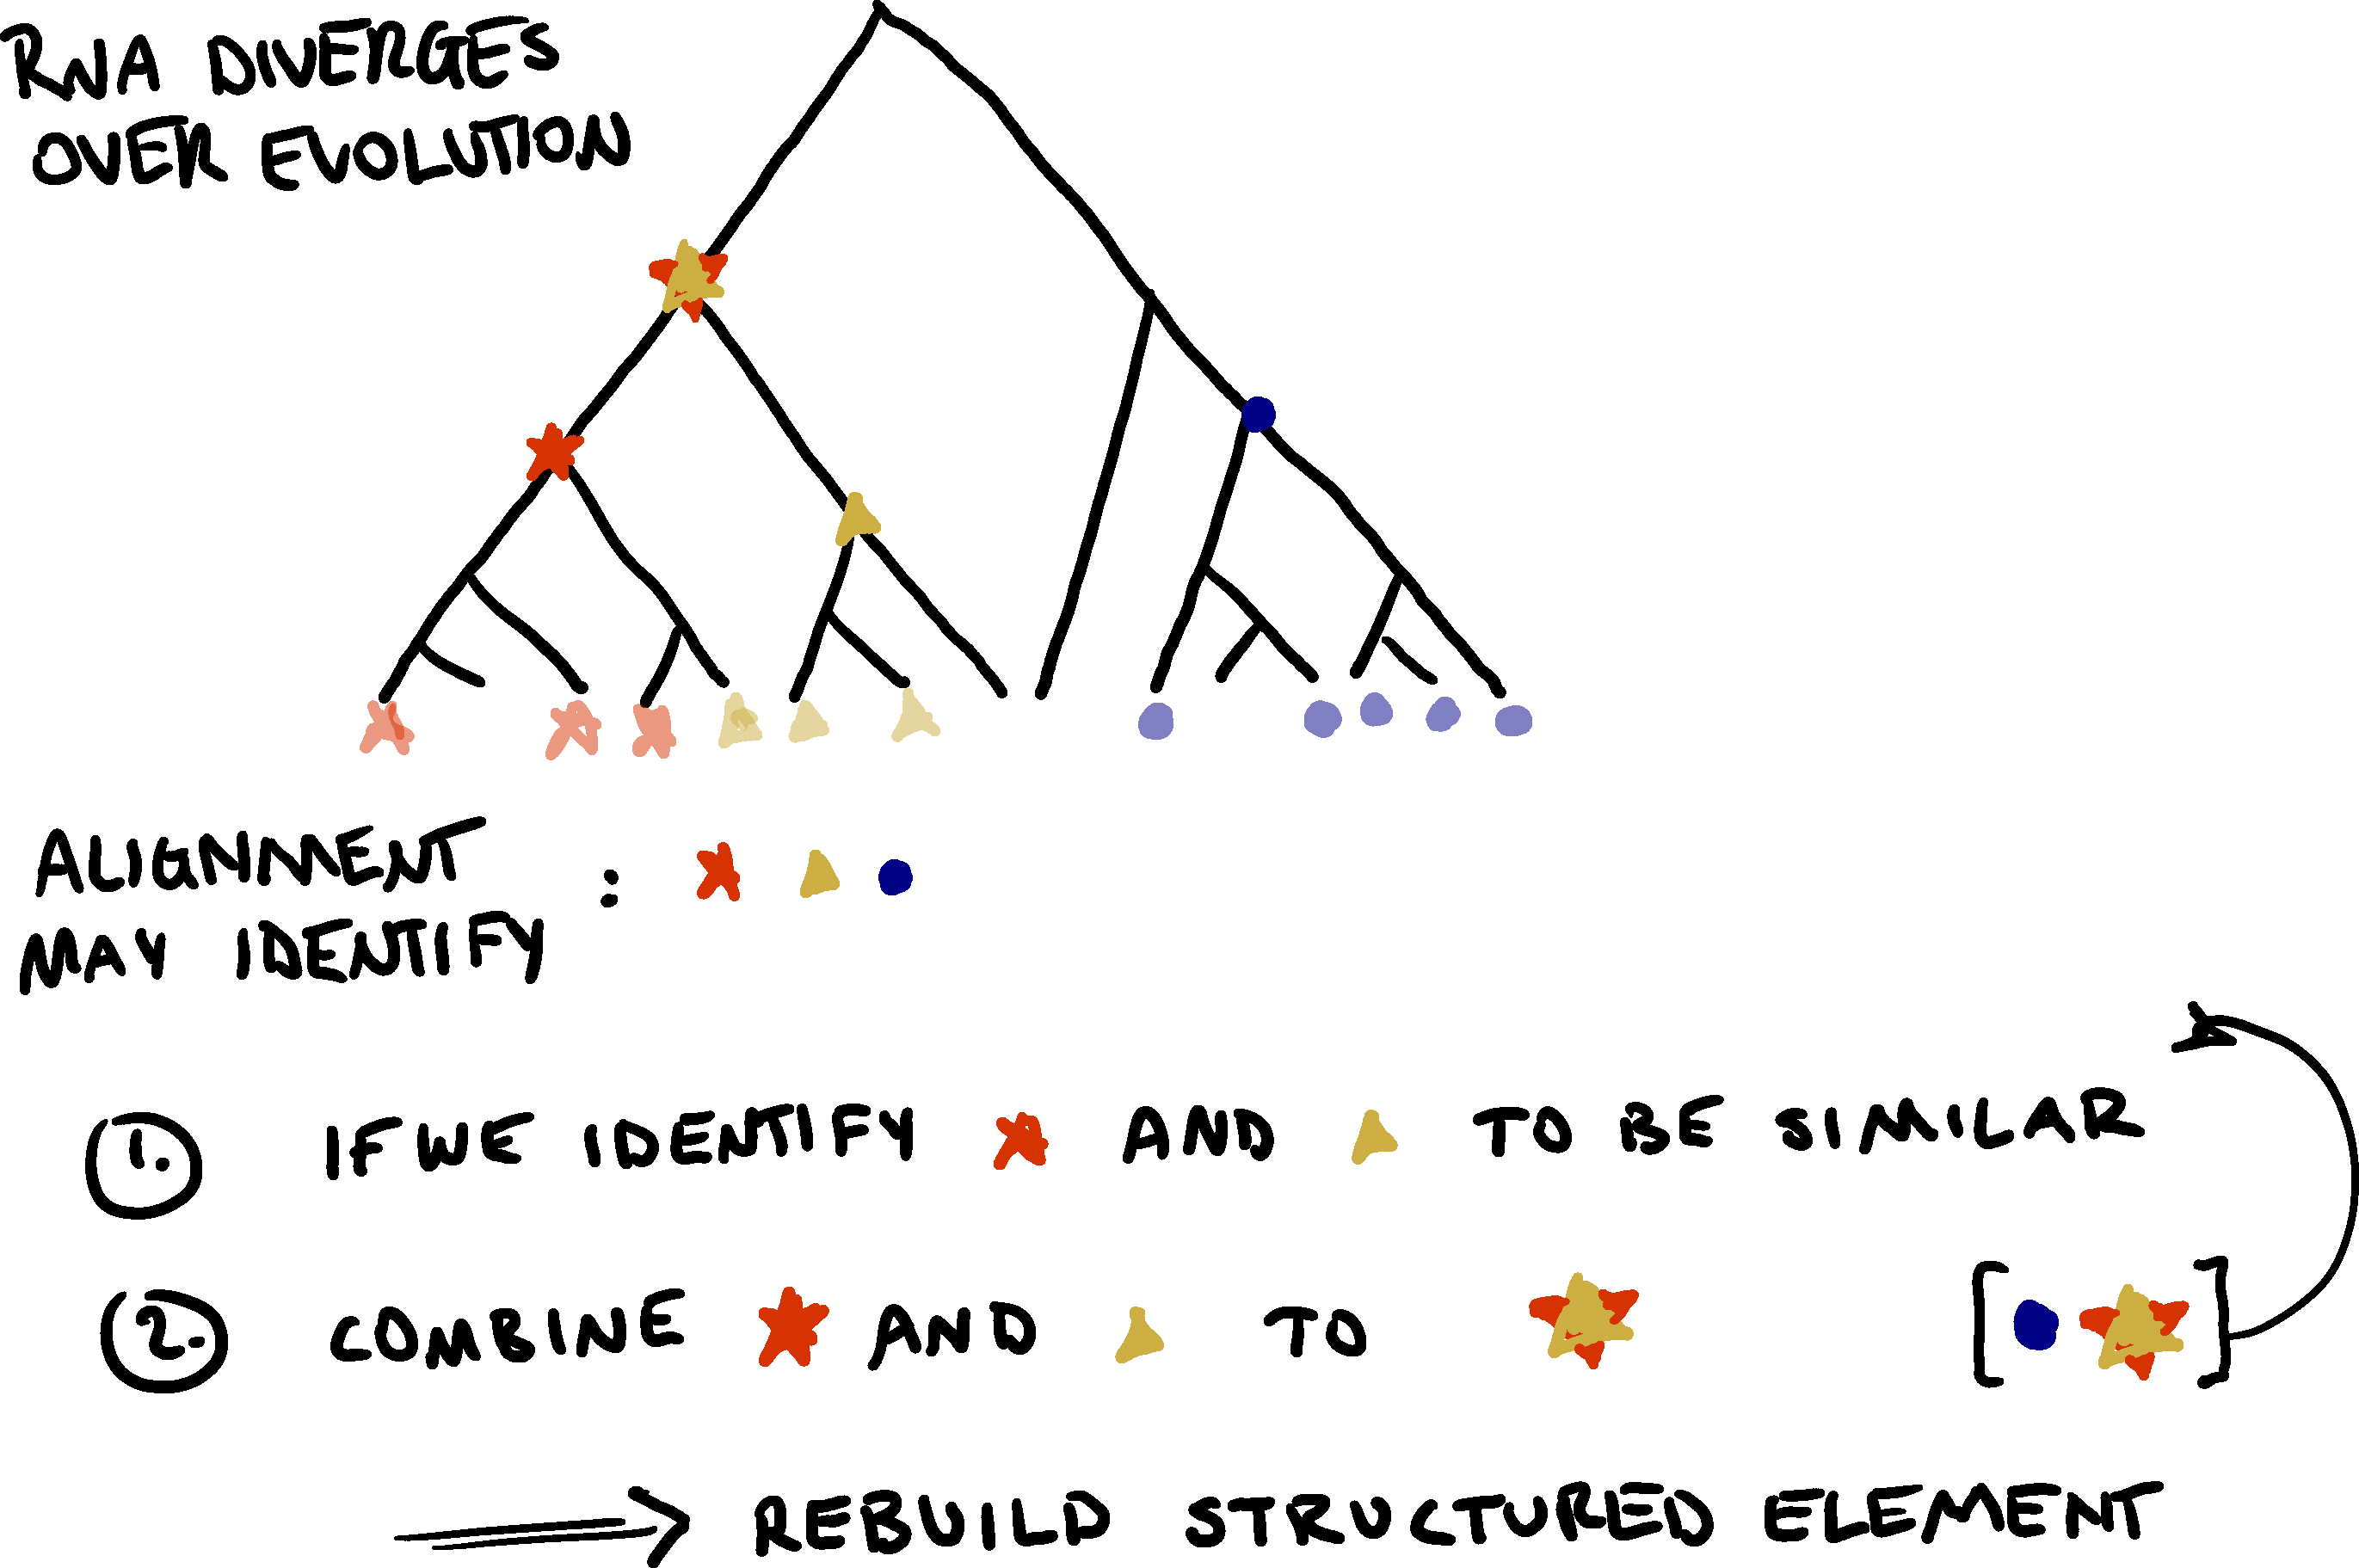
\includegraphics[width=0.8\textwidth]{figures/discussion/cluster-merging.pdf}
    \caption[Covariance model clustering and merging]{\textbf{Covariance model clustering and merging.} 
    Shown in red, gold and blue are structured RNA elements that have been identified by local alignment.
    Identified elements are homologous to each other, but are not similar enough to be detected by classical homology search methods.
    Covariance models describing these elements can be clustered based on their similarity, and merged to create a new model that captures the shared features of the original models. 
    This approach can be used to identify more distant homologs and improve the sensitivity of RNA discovery pipelines.}
    \label{fig:cluster-merging}
\end{figure}

The covariance model combination approach (Figure \ref{fig:cluster-merging}) was attempted in this project, but was not successful.
Implementation was attempted by aligning synthesised sequences from each model and then building a new model from the resulting alignment.
This was either done by aligning the sequences with a multiple sequence alignment tool, or by aligning the models with a covariance model alignment tool.
Testing was done with fractured \ac{FMN} riboswitch models.
The Rfam annotated \ac{FMN} seed sequences (Section~\ref{subsec:covariance-models}) were clustered, aligned, structure predicted and built into covariance models as in the final steps of the computational discovery pipeline (Sections~\ref{subsec:clustering}, \ref{subsec:rna-alignment}, \ref{subsec:covariance-analysis} and \ref{sec:build_cm}).
Models were then clustered and iteratively merged, and the resulting model was tested against the original \ac{FMN} riboswitch model.
Neither alignment method was successful in producing new models which scored well (with the combined \ac{KS} D value) against the original \ac{FMN} riboswitch model.
These results were preliminary and not reported.
Further work is needed to develop a reliable method for combining covariance models, and to test the resulting models against known structured RNA elements.
Also, compared to classical homology search methods, this approach is computationally expensive and time-consuming, and so may not be practical for large-scale RNA discovery pipelines.

\section{Conclusions}

The first aim of this project was to screen for conserved RNA structural elements located near the \ac{BLUF} domain.
This was achieved, and two candidate structured RNA elements were identified.
The candidates had weak covariation signal and low-confidence interaction predictions.
Further work is needed to validate these candidates, and to determine if they are functional RNAs or involved in light sensing.

The second aim was to develop a protein-first structured RNA discovery pipeline.
This was achieved, and the pipeline was tested with a positive control and a negative control set.
The positive control \ac{FMN} riboswitch was successfully recovered.
This showed the feasibility of a protein-first approach to RNA discovery.
The negative control set provided a baseline for the covariation signal expected when no known structured RNA is present.
Most negative control candidates were found to have weak covariation signal.
One candidate (flagellin candidate 327) produced a strong false-positive covariation signal, and was found to be a conserved protein-coding sequence rather than a structured RNA.
The pipeline is reusable and could be used to screen for conserved RNA structural elements associated with other protein domains in future work.

The third aim was to develop a method for clustering covariance models based on their similarity.
This was a later addition to the project, after realising that there was a gap in bioinformatic tools for a fast, working, reliable and statistically defensible similarity scoring.
Several approaches were developed and tested, all capable of clustering Rfam RNA families into their annotated clans (Table~\ref{tab:tab:classifier_comparison}).
Further work is needed to refine this clustering approach and to better validate it.

Overall, the aims of this project were achieved, and a reusable discovery pipeline was developed and tested.
There is some evidence for the use of a protein-first approach to RNA discovery, and the discovery pipeline could be used to screen for conserved RNA structural elements associated with other protein domains in future work.
Beyond this, there is value in finding structured RNA elements and gaining a better understanding of their biological roles, and in developing bioinformatic tools to support this work.

\section{Limitations}

Several limitations apply to the discovery pipeline and the results presented in this project.
The positive control was a single, relatively easy run: the \ac{FMN} riboswitch is highly conserved and well characterised, and the protein domain profile used as the anchor was generated from sequences neighbouring the Rfam-annotated riboswitch.
Recovery of this signal therefore represents a best-case scenario, and is not a general measure of the sensitivity of the pipeline to less conserved or more divergent RNAs.
The negative controls were imperfect, since a domain cannot be proven to lack an associated RNA, only four domains were tested in a single genus, and one of them (flagellin) is itself a less certain negative given reports of RNA regulation of flagellar genes \citet{Mika2013}.
One flagellin candidate scored highly but was protein-coding, so the covariation score alone cannot distinguish a structured RNA from a conserved coding sequence.
Overall, controls were limited, partially by the nature of discovery pipelines, but further work should include a larger set of positive and negative controls, and a more diverse set of protein domains and bacterial species.

The \ac{BLUF} search was restricted to a single genus, \emph{Burkholderia}, and the covariation signal for both \ac{BLUF}-associated candidates was weak.
For each candidate, the original or the iteratively expanded alignment was chosen according to which gave stronger covariation, which adds analytic flexibility.
AlphaFold~3 interface confidence scores (ipTM) were low for both candidates and for the positive control, so the predicted complexes provide no evidence of a specific interaction.
Finally, no experimental validation was performed, so the candidates should be regarded as hypotheses rather than confirmed functional RNAs.

Screening is also limited to just up and down stream of same strand, as we saw with the CRISPR-DR42 conserved RNA protein associations can go beyond this limited relationship.
The discovery pipeline could be extended to mine structured RNAs from more distant intergenic regions, and from the opposite strand to the protein coding gene.
Further, the pipeline currently only searches for structured RNAs associated with a single protein domain, but could be extended to search for structured RNAs associated with multiple protein domains, or with a combination of protein domains and other genomic features.

There are also limitations which arrise from the use of unreliable genome annotations.
The discovery pipeline relies on the accuracy of genome annotations and proteom translations to identify protein coding genes and their associated intergenic regions.
These are known to be error-prone\citep{Salzberg2019}, and despite filtering for contamination and completeness, it is likely that some of the genomes used in this project contain annotation errors.
It is possible these errors play at least some role in the lack of complete consensus on position relative to homologous protein coding gene for the tested riboswitch cases (Table~\ref{tab:results_summary}).

There will also be limitations in the homology searches, both from the protein domain profile searches and from the clustering and alignment steps.
Some of this is unavoidable and a result of the twilight zone of homology, where sequences are too divergent to be detected by homology search methods \citep{Rost1999,McGimpsey2019}.

Overall, there are many limitations to the discovery pipeline and the results presented in this project, but ultimately is intended to be a quick approach to checking for conserved RNA structural elements located near a protein domain of interest.
Once a candidate is identified, further work is needed to validate it and determine if it is a functional RNA or involved in the biological process of interest.

\section{Future directions}

\subsection{Discovery pipeline extension}

There are many ways in which the discovery pipeline could be extended and improved.
These include improving the tool selection, filtering steps and tool parameters for the discovery pipeline, and incorporating additional tools for structural clustering and alignment of RNA elements.
With a wider range of positive and negative controls, the discovery pipeline could be further optimised for speed and sensitivity.
This could introduce some bias in the way current curated RNA elements are identified and lead to overfitting, but would be a useful exercise to improve the discovery pipeline.

The covariance model clustering approach could be integrated into the discovery pipeline to identify similar covariance models and merge them to create a new model that captures the shared features of the original models.
This would allow for the identification of more distant homologs and improve the sensitivity of RNA discovery pipelines, and power of any covariance analysis.
The alignment and covariance analysis steps would not need to identify deep homology or strong covariation signal, as the clustering and merging of covariance models would allow for the identification of more distant homologs.

There may be other tools that could be used to improve the discovery pipeline, and the pipeline could be further optimised for speed and sensitivity.
A preprint from September 2026, \citet{Li2026}, describes a new approach to the discovery of RNA protein systems, using a large language model to identify non-coding elements coevolving with proteins.
Their apprach predicts pairwise interactions between nucleotides and proteins, and has had success with identifying known structured RNA elements and their associated proteins.
This approach could be used to identify targets for \ac{RNP} discovery, or this idea of coevolution could be incorporated into the discovery pipeline to improve the likelihood of finding functional \ac{RNP} systems.
Another tool, RNA-align \citep{Gong2019}, aligns RNA secondary structures and could be used to improve the clustering of candidate RNA elements.
\citet{McGimpsey2019} describe an iterative approach to homology search using nhmmer, which they found to lower the twilight zone of RNA homology.
This approach could be used to improve the sensitivity of the nucleotide homology searches in the discovery pipeline, and a similar approach could be taken for the protein domain profile searches.
Further works should explore the use of these tools in the discovery pipeline, and compare their performance to the current approach.

Further binary logic could be added to the discovery pipeline to filter candidates based on their genomic context, such as their proximity to other genes or regulatory elements.
For example, non coding regions that are located near one light related protein domain or another light related protein domain, or one pathway related protein and a different pathway related protein.
This could be used to identify candidates in a more complex biology aware manner.

\subsection{Further targets for \ac{RNP} discovery}

There are endless possibilities for further targets for \ac{RNP} discovery, and the discovery pipeline could be applied to a wide range of protein domains and biological processes.
Expand beyond \ac{BLUF}, other light-pathway anchors (e.g. phytochromes, cryptochromes) and other photoreceptor families could be used to anchor searches for further \ac{RNP} or cis-regulatory candidates.
These searches could be extended to other bacterial species, and to other kingdoms of life, including archaea and eukaryotes.

With the success of \citet{Durrant2024} in identifying the novel Bridge RNA recombinase system, TIGR from \citet{Bruck2025}, and the earlier discovery of \ac{CRISPR} \citep{Barrangou2007}, it would be interesting to apply the discovery pipeline to other DNA editing proteins.
\ac{RNP} complex discoveries like this have the potential to be significant biotechnological tools, as the previous examples highlight.

\subsection{Experimental validation}

Once a candidate structured RNA element is identified, and further investigated by computational methods, it should be experimentally validated.
Neither of the \ac{BLUF}-associated candidates identified in this project are currently particularly convincing as structured RNA elements, but if further work found more evidence for them, or if other candidates were identified, they should be experimentally validated.
Chemical probing methods, such as \ac{SHAPE-seq} \citep{Lucks2011} or \ac{DMS-MaPseq} \citep{Zubradt2017}, could be used to determine the secondary structure of the RNA element.
Also, depending on the predicted function of the RNA element, experimental assays could be used to determine its biological role, such as real time quantitative \ac{PCR} and stimulus-response experiments for cis-regulatory elements.




\cleardoublepage
\bibliographystyle{cell}
\bibliography{references}

\chapter{Appendices}

\section{Code and Data Availability}
\label{sec:code-and-data-availability}

Code is available from:

\begin{itemize}
    \item \url{https://github.com/dan-432/DarwinsRNAHunt} contains the positive control and discovery snakemake pipelines and associated analyses.
    \item \url{https://github.com/dan-432/cm-iterative-expansion} contains the logic for and analysis of the itertive expansion of candidate \ac{CM}s.
    \item \url{https://github.com/dan-432/cm-simile} contains the logic for and analysis of the pairwise similarity scoring of candidate \ac{CM}s
\end{itemize}

See top-level README files for further documentation on file structure and running instructions.

Data and computed results are available from \dots

[link to zenodo]

\section{Supplimentary Tables}

\begingroup
\footnotesize
\begin{longtable}{p{0.14\textwidth}p{0.50\textwidth}}
\caption[Positive controls (RNA $\rightarrow$ protein)]{Rfam families used as positive controls for the RNA-to-protein direction.}
\label{tab:positive_controls_input} \\
\hline
Rfam ID & Description \\
\hline
\endfirsthead
\multicolumn{2}{c}{\tablename\ \thetable{} -- continued} \\
\hline
Rfam ID & Description \\
\hline
\endhead
\hline
\multicolumn{2}{r}{\emph{Continued on next page}} \\
\endfoot
\hline
\endlastfoot
RF01315 & CRISPR RNA direct repeat element \\
RF00050 & FMN riboswitch \\
RF00162 & SAM riboswitch \\
RF01734 & Fluoride riboswitch \\
\end{longtable}
\endgroup

\begin{table}[H]
\centering
\caption[Filtering thresholds used in the computational discovery pipeline]{\textbf{Filtering thresholds used in the computational discovery pipeline.}
    The discovery pipeline was run with these filtering thresholds to identify candidate structured RNA elements associated with the \ac{BLUF} protein domain.
    These thresholds were guided by poitive and negative control experiments.}
\label{tab:thresholds}
\begin{tabular}{@{}lll@{}}
\toprule
Step & Parameter & Value \\
\midrule
3.1 Domain search & hmmsearch E-value & $\leq 10^{-5}$ \\
3.2 Flanking extraction & Minimum length & 20\,nt \\
 & Overlap into coding sequence & 5\,nt \\
3.3 Clustering & mmseqs2 minimum sequence identity & 0.4 \\
 & Coverage (mode 3) & $\geq 0.5$ \\
 & Minimum cluster size & 5 \\
 & Trimming padding & 15\,nt \\
3.5 Covariance analysis & R-scape E-value (at least one covarying pair) & $\leq 0.05$ \\
3.6 Calibration & Random sequence length & $0.8$ megabases \\
\bottomrule
\end{tabular}
\end{table}

\begingroup
\footnotesize
\begin{longtable}{p{0.14\textwidth}p{0.36\textwidth}p{0.24\textwidth}p{0.17\textwidth}}
\caption[Discovery pipeline inputs (protein $\rightarrow$ RNA)]{\textbf{Inputs to the protein-to-RNA discovery pipeline}: protein domain (or protein cluster), description, and the GTDB bacterial clade searched. Genomes were filtered at 99.9\% completeness and $\le$1\% contamination for every pair.}
\label{tab:discovery_inputs} \\
\hline
Domain ID & Description & Bacterial taxon (GTDB node) & Role \\
\hline
\endfirsthead
\multicolumn{4}{c}{\tablename\ \thetable{} -- continued} \\
\hline
Domain ID & Description & Bacterial taxon (GTDB node) & Role \\
\hline
\endhead
\hline
\multicolumn{4}{r}{\emph{Continued on next page}} \\
\endfoot
\hline
\endlastfoot
IPR005594 & SecY domain & \emph{f\_\_Burkholderiaceae\_C} (36.0) & Negative control \\
IPR002208 & YadA-like membrane anchor domain & \emph{f\_\_Burkholderiaceae\_C} (36.0) & Negative control \\
IPR021309 & YgaP-like transmembrane domain & \emph{f\_\_Burkholderiaceae\_C} (36.0) & Negative control \\
IPR001029 & Bacterial flagellin N-terminal helical region & \emph{f\_\_Burkholderiaceae\_C} (36.0) & Initially as negative control \\
IPR007024 & BLUF domain & \emph{f\_\_Burkholderiaceae\_C} (36.0) & Test target \\
cluster\_1341 & FMN riboswitch control (protein cluster) & \emph{f\_\_Microbacteriaceae} (100) & Positive control \\
CRISPR\_Cas2 & CRISPR RNA direct repeat element control (Cas2) & \emph{o\_\_Lactobacillales} (92.0) & Positive control \\
\end{longtable}
\endgroup


\begingroup
\scriptsize
\setlength{\tabcolsep}{2pt}
\begin{longtable}{lrrrlrrrrrrr}
\caption[Positive control run clusters (full)]{Top 10 clusters by genome spread for each RNA family.}
\label{tab:cluster_appendix} \\
\hline
Cluster & Genomes & Seqs & Prev. & Position & Up. & Cont. & Strand & Interg. & Purity \\
\hline
\endfirsthead

\multicolumn{12}{c}{\tablename\ \thetable{} -- continued} \\
\hline
Cluster & Genomes & Seqs & Prev. & Position & Up. & Cont. & Strand & Interg. & Purity \\
\hline
\endhead

\hline
\multicolumn{12}{r}{\emph{Continued on next page}} \\
\endfoot

\hline
\endlastfoot

\multicolumn{12}{l}{\textbf{FMN riboswitch (RF00050)}: 1599 clusters, 2009 genomes, 1115 singleton-genome clusters} \\
\hline
204$^\dagger$ & 926 & 934 & 0.4609 & Up 1 & 0.913 & 0.007 & 1.0 & 0.979 & 0.4609 \\
695 & 578 & 748 & 0.2877 & Up 1 & 0.999 & 0.003 & 1.0 & 0.979 & 0.288 \\
600 & 409 & 417 & 0.2036 & Up 1 & 1.0 & 0.01 & 1.0 & 0.981 & 0.3223 \\
89 & 295 & 295 & 0.1468 & Up 1 & 1.0 & 0.01 & 1.0 & 0.98 & 0.147 \\
58 & 189 & 189 & 0.0941 & Down 1 & 0.0 & 0.0 & 1.0 & 0.979 & 0.1547 \\
340 & 188 & 188 & 0.0936 & Up 1 & 1.0 & 0.005 & 1.0 & 0.973 & 0.2709 \\
1453 & 119 & 119 & 0.0592 & Down 2 & 0.0 & 0.0 & 1.0 & 0.975 & 0.1941 \\
100 & 96 & 99 & 0.0478 & Down 1 & 0.111 & 0.0 & 0.869 & 1.0 & 0.0478 \\
1501 & 90 & 93 & 0.0448 & Down 1 & 0.462 & 0.0 & 0.72 & 0.935 & 0.0448 \\
113 & 71 & 71 & 0.0353 & Up 1 & 1.0 & 0.0 & 0.0 & 0.958 & 0.7474 \\
\hline

\multicolumn{12}{l}{\textbf{SAM riboswitch (RF00162)}: 2247 clusters, 1535 genomes, 1553 singleton-genome clusters} \\
\hline
831$^\dagger$ & 634 & 873 & 0.413 & Up 1 & 0.885 & 0.006 & 0.982 & 0.976 & 0.413\\
252 & 448 & 450 & 0.2919 & Up 1 & 0.847 & 0.082 & 0.98 & 0.913 & 0.2919 \\
2042 & 406 & 413 & 0.2645 & Up 1 & 0.961 & 0.0 & 0.884 & 0.99 & 0.2645 \\
1591 & 401 & 412 & 0.2612 & Up 1 & 0.993 & 0.005 & 0.993 & 0.973 & 0.2612 \\
1392 & 361 & 586 & 0.2352 & Up 1 & 0.931 & 0.015 & 0.945 & 0.966 & 0.2352 \\
2115 & 262 & 304 & 0.1707 & Up 1 & 0.947 & 0.013 & 0.977 & 0.961 & 0.1707 \\
1725 & 198 & 198 & 0.129 & Up 1 & 1.0 & 0.0 & 0.0 & 0.864 & 0.3984 \\
1834 & 134 & 134 & 0.0873 & Up 1 & 1.0 & 0.0 & 0.0 & 1.0 & 0.0873 \\
1517 & 116 & 138 & 0.0756 & Up 1 & 0.992 & 0.058 & 1.0 & 0.935 & 0.0756 \\
833 & 98 & 99 & 0.0638 & Down 1 & 0.0 & 0.0 & 1.0 & 0.96 & 0.5904 \\
\hline

\multicolumn{12}{l}{\textbf{CRISPR-DR42 (RF01351)}: 394 clusters, 65 genomes, 340 singleton-genome clusters} \\
\hline
294$^\dagger$ & 28 & 264 & 0.4308 & Down 1 & 0.011 & 0.0 & 0.0 & 0.989 & 0.4308 \\
217 & 27 & 192 & 0.4154 & Down 2 & 0.068 & 0.0 & 0.0 & 0.99 & 0.4154 \\
134 & 24 & 419 & 0.3692 & Up 1 & 0.577 & 0.007 & 0.024 & 0.981 & 0.3692 \\
162 & 7 & 65 & 0.1077 & Down 1 & 0.0 & 0.0 & 0.015 & 1.0 & 0.1077 \\
121 & 6 & 238 & 0.0923 & Up 1 & 0.542 & 0.0 & 0.891 & 1.0 & 0.1364 \\
161 & 6 & 69 & 0.0923 & Up 1 & 0.565 & 0.0 & 0.188 & 1.0 & 0.1364 \\
301 & 5 & 37 & 0.0769 & Up 1 & 1.0 & 0.0 & 0.0 & 1.0 & 0.0769 \\
120 & 4 & 34 & 0.0615 & Down 1 & 0.0 & 0.0 & 0.735 & 1.0 & 0.0615 \\
136 & 4 & 12 & 0.0615 & Down 2 & 0.25 & 0.0 & 0.333 & 1.0 & 0.0615 \\
253 & 4 & 20 & 0.0615 & Up 1 & 0.85 & 0.0 & 0.7 & 1.0 & 0.0615 \\
\hline

\multicolumn{12}{l}{\textbf{Fluoride riboswitch (RF01734)}: 951 clusters, 661 genomes, 779 singleton-genome clusters} \\
\hline
761$^\dagger$ & 259 & 345 & 0.3918 & Up 1 & 0.974 & 0.014 & 0.977 & 0.939 & 0.39248 \\
453 & 254 & 269 & 0.3843 & Up 1 & 0.992 & 0.019 & 0.981 & 0.944 & 0.3848 \\
768 & 73 & 89 & 0.1104 & Up 2 & 0.909 & 0.011 & 0.91 & 0.899 & 0.1106 \\
561 & 64 & 65 & 0.0968 & Up 1 & 1.0 & 0.062 & 1.0 & 0.877 & 0.2623 \\
136 & 33 & 43 & 0.0499 & Up 1 & 0.814 & 0.0 & 0.744 & 0.977 & 0.05 \\
11 & 28 & 39 & 0.0424 & Up 1 & 0.895 & 0.026 & 0.795 & 0.949 & 0.0424 \\
577 & 21 & 28 & 0.0318 & Up 1 & 1.0 & 0.036 & 0.643 & 0.929 & 0.0318 \\
169 & 19 & 20 & 0.0287 & Down 1 & 0.4 & 0.0 & 0.75 & 0.85 & 0.0288 \\
526 & 18 & 23 & 0.0272 & Up 1 & 0.739 & 0.0 & 0.87 & 0.913 & 0.0272 \\
279 & 17 & 17 & 0.0257 & Up 1 & 0.941 & 0.0 & 0.059 & 0.824 & 0.0258 \\
\end{longtable}
\endgroup

\vspace{4pt}
\noindent\footnotesize Genomes/Seqs: number of genomes/sequences in the cluster; Prev.: fraction of available genomes containing the cluster; Position: dominant position relative to the nearest gene (upstream/downstream and gene rank); Up., Cont., Strand, Interg.: fraction of sequences upstream of, contained within, on the same strand as, and fully intergenic relative to that gene; Purity: clade purity; All clusters were polyphyletic. $\dagger$ marks clusters with an InterProScan hit (see Table~\ref{tab:results_summary}).

\begingroup
\footnotesize
\begin{longtable}{p{0.13\textwidth}rrrrp{0.19\textwidth}p{0.12\textwidth}p{0.13\textwidth}}
\caption[Full covariation results for FMN Riboswitch rediscovery]{Full R-scape covariation results and pairwise identity summary for FMN riboswitch rediscovery, and for the Rfam-annotated true-positive alignment.}
\label{tab:rscape_appendix} \\
\hline
Candidate & Cov.\ pairs$^{*}$ & True & FP & E-value range & \% id.\ true pos. & \% id.\ nearest \\
\hline
\endfirsthead
\multicolumn{7}{c}{\tablename\ \thetable{} -- continued} \\
\hline
Candidate & Cov.\ pairs$^{*}$ & True & FP & E-value range & \% id.\ true pos. & \% id.\ nearest \\
\hline
\endhead
\hline
\multicolumn{7}{r}{\emph{Continued on next page}} \\
\endfoot
\hline
\endlastfoot
\emph{fmn\_cm\_on\_micro (positive control)} & 11 & 42 & 0 & $[-9.95,\,874.13]$ & 100.00 & 80.36 (379) \\
416 & 30 & 46 & 0 & $[-9.95,\,916.18]$ & 76.75 & 94.87 (531) \\
647 & 30 & 52 & 0 & $[-9.95,\,923.72]$ & 67.99 & 96.65 (491) \\
35  & 27 & 60 & 0 & $[-9.95,\,903.89]$ & 75.02 & 92.87 (379) \\
379 & 26 & 59 & 0 & $[-9.95,\,909.40]$ & 80.36 & 92.87 (35) \\
491 & 27 & 62 & 0 & $[-9.95,\,917.35]$ & 67.95 & 96.65 (647) \\
40  & 17 & 43 & 0 & $[-9.95,\,918.20]$ & 74.41 & 92.95 (531) \\
384 & 22 & 57 & 0 & $[-9.95,\,934.88]$ & 68.73 & 94.06 (647) \\
539 & 14 & 38 & 0 & $[-9.95,\,898.55]$ & 76.99 & 87.36 (384) \\
531 & 13 & 41 & 0 & $[-9.95,\,910.91]$ & 78.73 & 94.87 (416) \\
396 & 8  & 39 & 0 & $[-9.95,\,822.31]$ & 0.00  & 90.79 (109) \\
109 & 5  & 26 & 0 & $[-9.95,\,829.86]$ & 0.00  & 90.79 (396) \\
442 & 2  & 18 & 0 & $[-9.95,\,491.32]$ & 0.00  & 9.71 (396) \\
\end{longtable}
\endgroup

\vspace{4pt}
\noindent\footnotesize $^{*}$ Number of covarying base pairs identified by R-scape at $E \le 0.05$; equal to true positives (TP) since FP\,=\,0 for all alignments.

\begin{longtable}{@{}p{0.18\textwidth}p{0.22\textwidth}p{0.52\textwidth}@{}}
\caption{My table caption}\label{tab:mytable} \\
\toprule
\textbf{ID} & \textbf{Description} & \textbf{Sequence} \\
\midrule
\endfirsthead

\multicolumn{3}{c}{\tablename\ \thetable{} -- continued} \\
\toprule
\textbf{ID} & \textbf{Description} & \textbf{Sequence} \\
\midrule
\endhead

\midrule
\multicolumn{3}{r}{\textit{Continued on next page}} \\
\endfoot

\bottomrule
\endlastfoot

\multicolumn{3}{@{}l}{\textit{cds-APW43854.1|utr3|CP019239.1:3318396-3318523(-)}} \\
 & Representative from Bluf downstream candidate 130 & \\
 & RNA & \seqsplit{ACGUGGCCCCCACGCUCCGCCGCUGCGCGGGUCGCUGCCCCCCGGGGGGGCUAAUUUGGCUUCGCCGCGCUUCGCGAGCCCUUGGGGCGGCCCGGCGGGAAAUUGCCUUUCCUUCCUCCGUCUACUGA} \\
 & Protein & \seqsplit{MLVRLLYASRAIDSRPDAIEAILTQSRNYNPSCGITGILCYGGGIFLQAIEGGRMAVSELYGHIQKDARHKDVVLLHYEEISERRFGGWTMGQVNMSKINTNILLKYAEKPELDPYSVSGKVSLALLEELMATASIIGRA} \\
\addlinespace[6pt]
\midrule

\multicolumn{3}{@{}l}{\textit{cds-MFN4120999.1|utr3|JBKBKQ010000028.1:10309-10517(-)}} \\
 & Rep from candidate cluster 332 & \\
 & RNA & \seqsplit{AAAGCGGGGCGCUUUGCUACUGCGCCAGCCGGUUCCGGGCCUGCUGUGCUCGCCGUACAGGAGUACGGCUGCGCGCAUCGACCCAGACUAGGCUGGCUCGCUACACAAAUCGCCCCACCUUUCUUCGCAGUCAUCCAUCACGGUUCGUAGCCGCAGCCGCCUAGAAGGCGCUGCGGCUUUUCUGUUCAGGCCGUUCUUUUUCUCGCCCG} \\
 & Protein & \seqsplit{MLVRLLYASRAVDTSPEAIEAILTQSRQHNPGSGITGVLCYGGGVFLQAIEGGRSAVSELYGHIQKDARHKNVELLHYEEISERRFGGWTMGQVNLSKINHSILLKYSEKPELDPYAVSGKVSFALLEELMATASIIGRA} \\
\addlinespace[6pt]
\midrule

\multicolumn{3}{@{}l}{\textit{BNBA01000017.1/83078-82865 --- unrelated fmn riboswitch sequence (negative control)}} \\
 & RNA & \seqsplit{GAACGUCUUCAGGGCGGGGUGAGAUUCCCCACCGGCGGUAGGUGCGGCGCCCUUGCGGCGAGGCACGAGCCCGCGAGCGCUUUCGAUGGCAUGCGAUCACGCCCCGCCGCGUGGGUCCGUGCCUUGGAAGGUCAGCAGAUCCGGUCAGAUGCCGGAGCCGACGGUCGGCAGGGCCCGGGGCCAUGCCGGAAAGUCCGGAUGAAAGAAGACGGUA} \\
 & BLUF protein & \seqsplit{MLVRLLYASRAVDTSPEAIEAILTQSRQHNPGSGITGVLCYGGGVFLQAIEGGRSAVSELYGHIQKDARHKNVELLHYEEISERRFGGWTMGQVNLSKINHSILLKYSEKPELDPYAVSGKVSFALLEELMATASIIGRA} \\
\end{longtable}

\begin{table}[H]
\centering
\footnotesize
\caption{Candidate clusters from the flagellin (IPR001029, PF00669) motif screen. Unlike the negative controls in Table~\ref{tab:negative_control_appendix}, this domain has a described precedent for associated \emph{cis}-regulatory elements coupling flagellar gene expression to assembly state (discussed in Section~\ref{sec:discussion}).}
\label{tab:flagellin_appendix}
\begin{tabular}{p{0.10\textwidth}p{0.14\textwidth}p{0.12\textwidth}p{0.08\textwidth}p{0.10\textwidth}p{0.10\textwidth}}
\hline
\textbf{Cluster} & \textbf{Direction} & \textbf{Cov.\ pairs$^{*}$} & \textbf{True} & \textbf{Sen.\ (\%)} & \textbf{F-score} \\
\hline
327 & Downstream & 11 & 40  & 27.50 & 43.14 \\
545 & Downstream & 2  & 48  & 4.17  & 8.00 \\
589 & Downstream & 4  & 103 & 3.88  & 7.48 \\
16  & Upstream   & 1  & 41  & 2.44  & 4.76 \\
265 & Downstream & 1  & 36  & 2.78  & 5.41 \\
725 & Downstream & 1  & 45  & 2.22  & 4.35 \\
161 & Downstream & 1  & 77  & 1.30  & 2.56 \\
272 & Downstream & 1  & 79  & 1.27  & 2.50 \\
214 & Upstream   & 1  & 165 & 0.61  & 1.20 \\
\hline
\end{tabular}

\par\smallskip
\begin{minipage}{\textwidth}
\raggedright
$^{*}$ Number of covarying base pairs identified by R-scape at $E \le 0.05$; equal to true positives (TP) since FP\,=\,0 in all cases.
\end{minipage}
\end{table}

\section{Supplimentary Figures}

\begin{figure}[H]
    \centering
    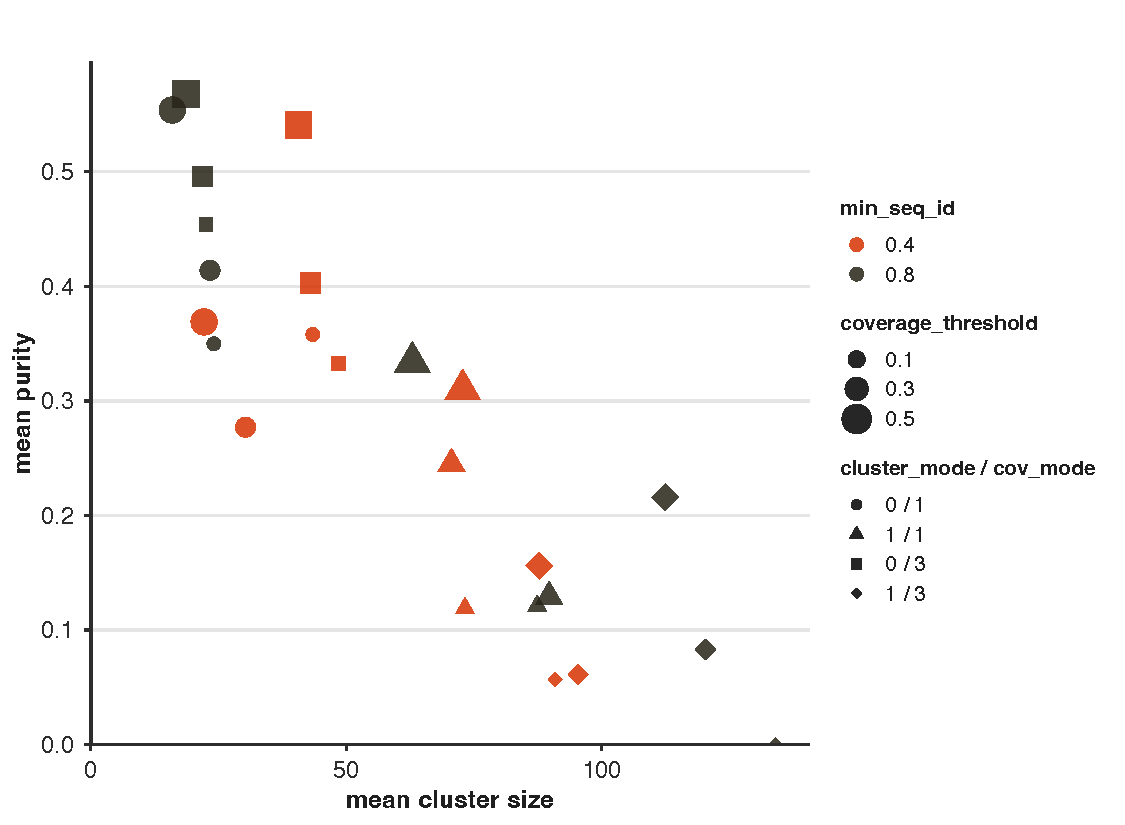
\includegraphics[width=0.95\textwidth]{figures/methods/tradeoff.pdf}
    \caption[Clustering parameter selection for positive control pipeline]{\textbf{Clustering parameter selection for positive control pipeline.}
    The clustering step of the positive control pipeline was run with a range of parameters, and the number of clusters and singleton-genome clusters were recorded.}
    \label{fig:poscontrol-clustering}
\end{figure}

\begin{figure}[H]
  \centering
  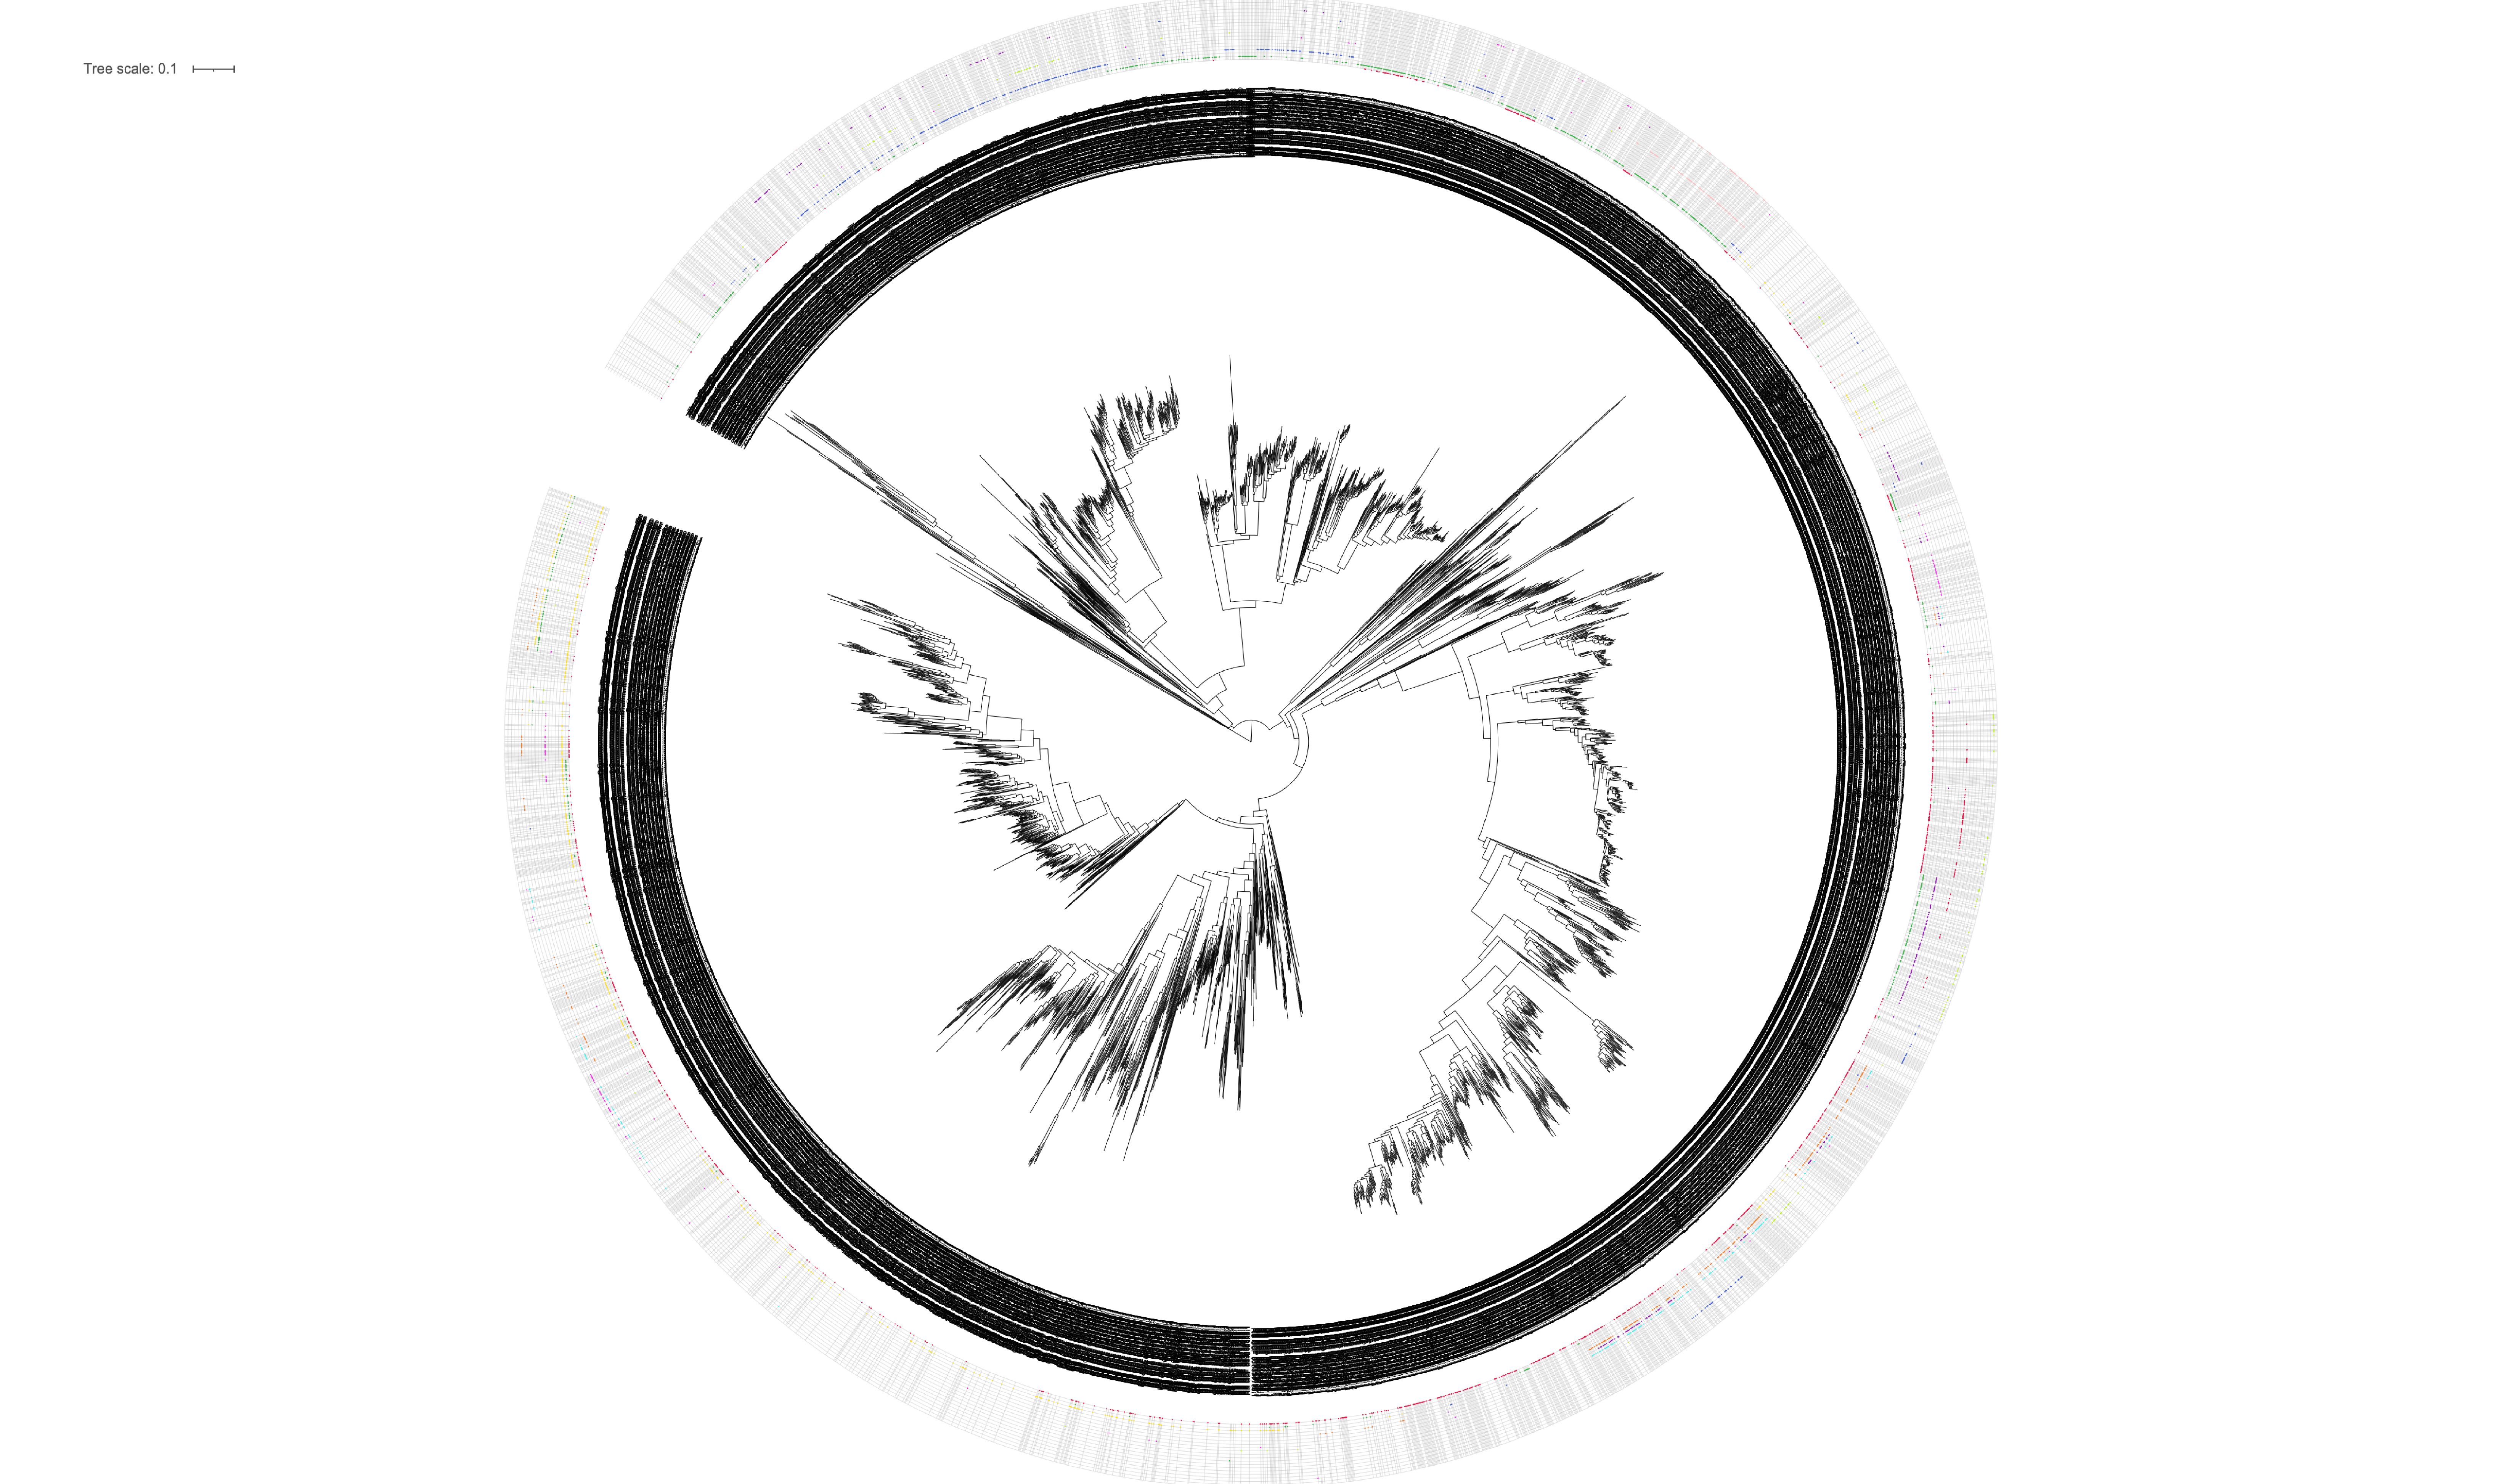
\includegraphics[width=0.95\textwidth]{figures/results/iTOL-gtdbtree-RF00050-clusterannotated.pdf}
  \caption[Prevalence of homologous protein sequences neighbouring \ac{FMN} riboswitch]{\textbf{Prevalence of homologous protein sequences neighbouring \ac{FMN} riboswitch.}
  Top 10 clusters by presence per genome are shown around tree, in order of Appendix Table \ref{tab:cluster_appendix}.
  Tree is annotated with analysis output of the positive control preperation pipeline output.
  It shows the \ac{GTDB} species taxonomy of representative genomes containing the \ac{FMN} riboswitch (as annotated by Rfam).}
  \label{fig:fmn-itol-tree}
\end{figure}

\begin{figure}[H]
  \centering
  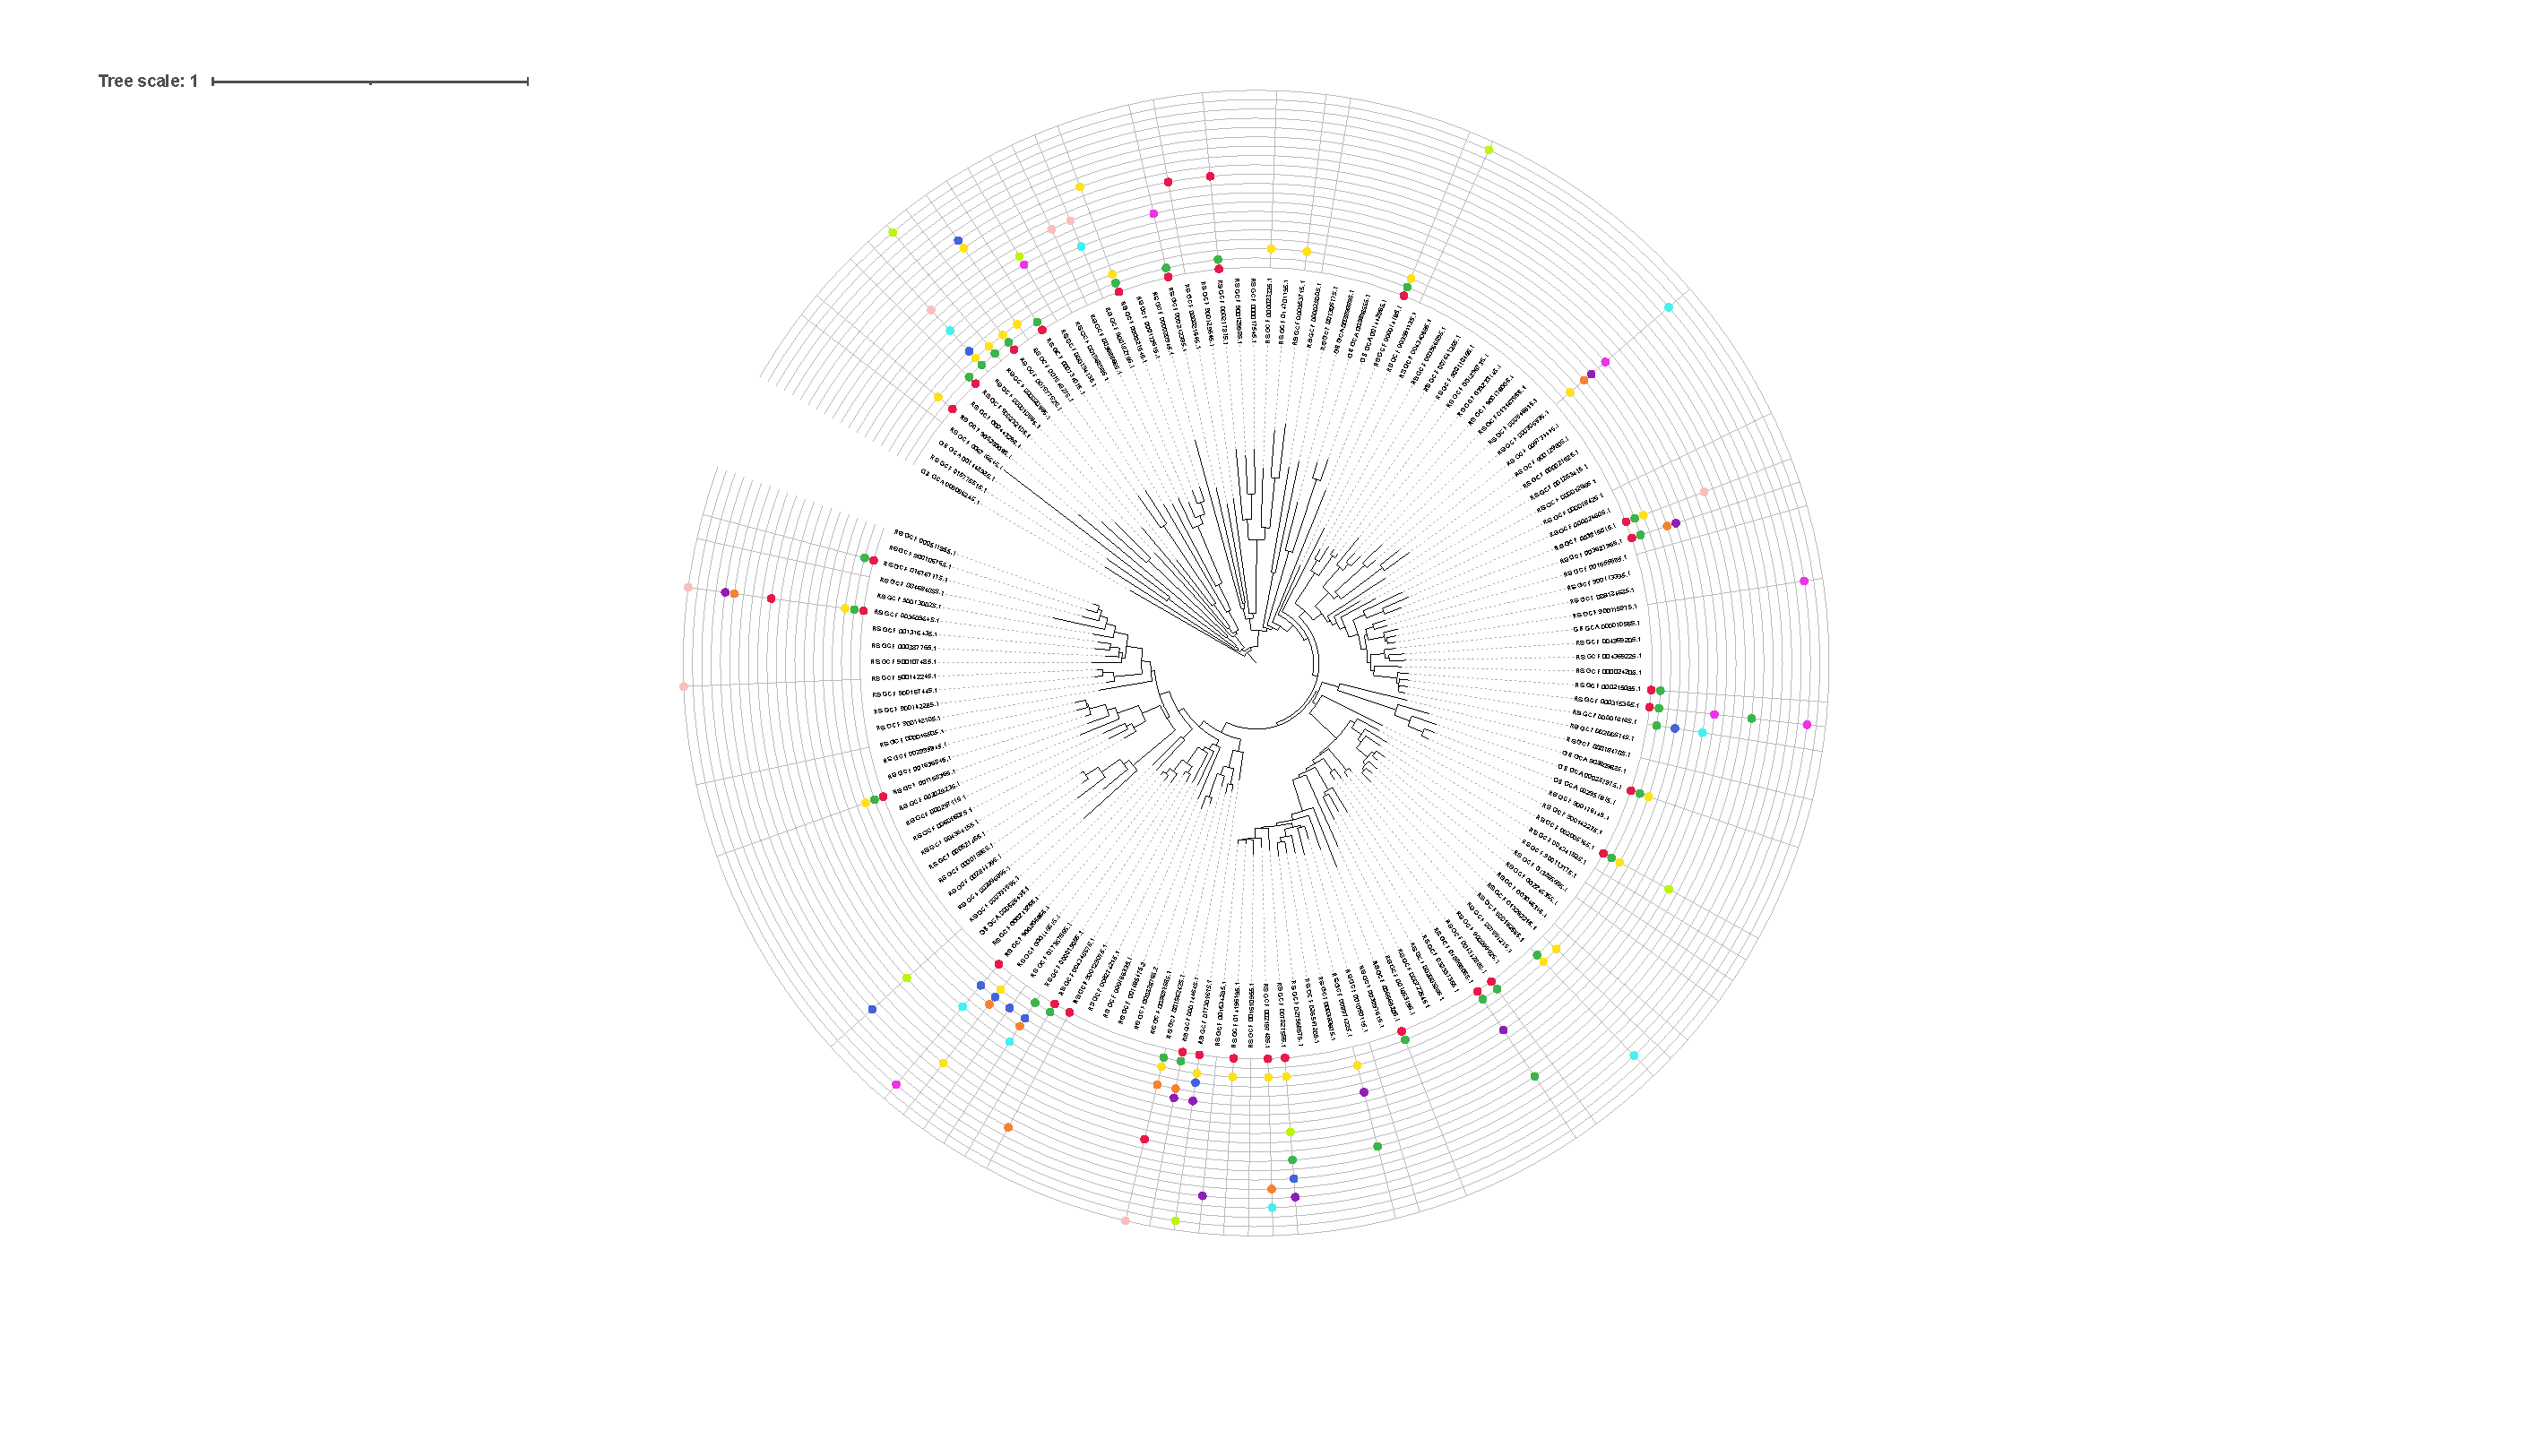
\includegraphics[width=0.95\textwidth]{figures/results/crisprrepeatelementtree.pdf}
  \caption[Prevalence of homologous protein sequences neighbouring \ac{CRISPR}-Direct Repeat 42]{\textbf{Prevalence of homologous protein sequences neighbouring \ac{CRISPR}-Direct Repeat 42.}
  Top 10 clusters by presence per genome are shown around tree, in order of Appendix Table \ref{tab:cluster_appendix}.
  Tree is annotated with analysis output of the positive control preperation pipeline output.
  It shows the \ac{GTDB} species taxonomy of representative genomes containing \ac{CRISPR}-Direct Repeat 42 (as annotated by Rfam).}
  \label{fig:cdr-itol-tree}
\end{figure}

\begin{figure}[p]
    \centering
    \begin{subfigure}[t]{0.48\textwidth}
        \centering
        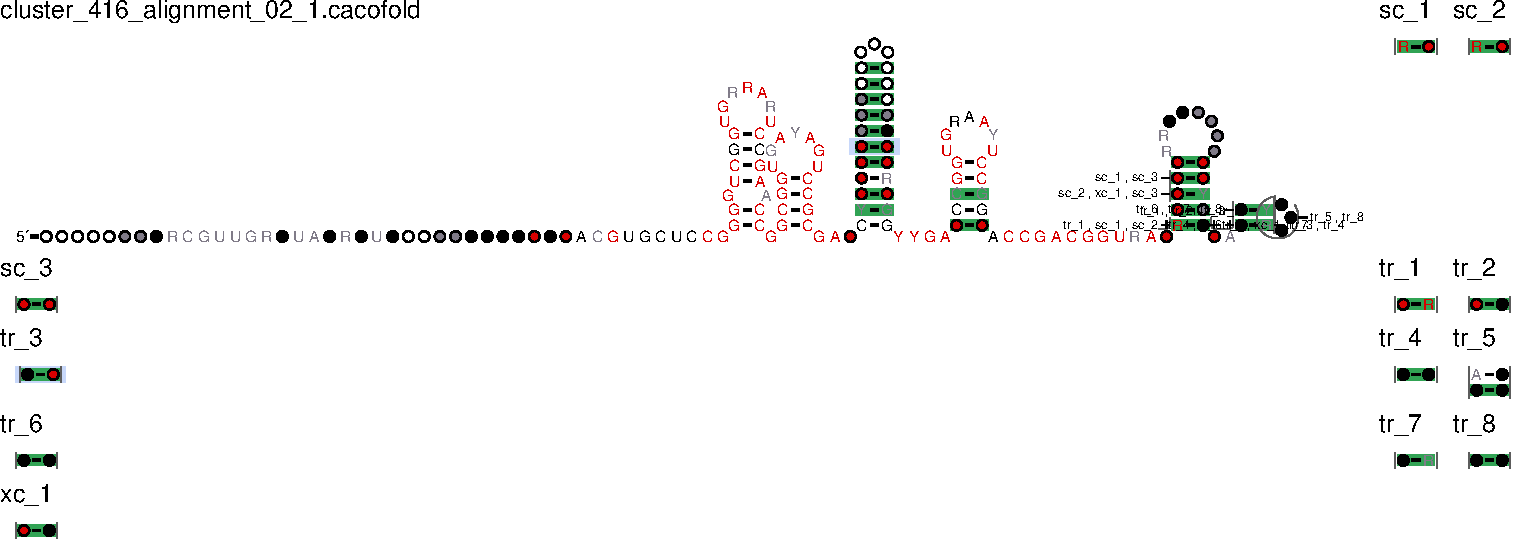
\includegraphics[width=\linewidth]{figures/results/drh-iteritive-expansion-structures/cluster_416_alignment_02_1.cacofold.R2R.sto.pdf}
        \caption{Candidate 416 (F = 78.95)}
        \label{fig:cand416-struct}
    \end{subfigure}
    \hfill
    \begin{subfigure}[t]{0.48\textwidth}
        \centering
        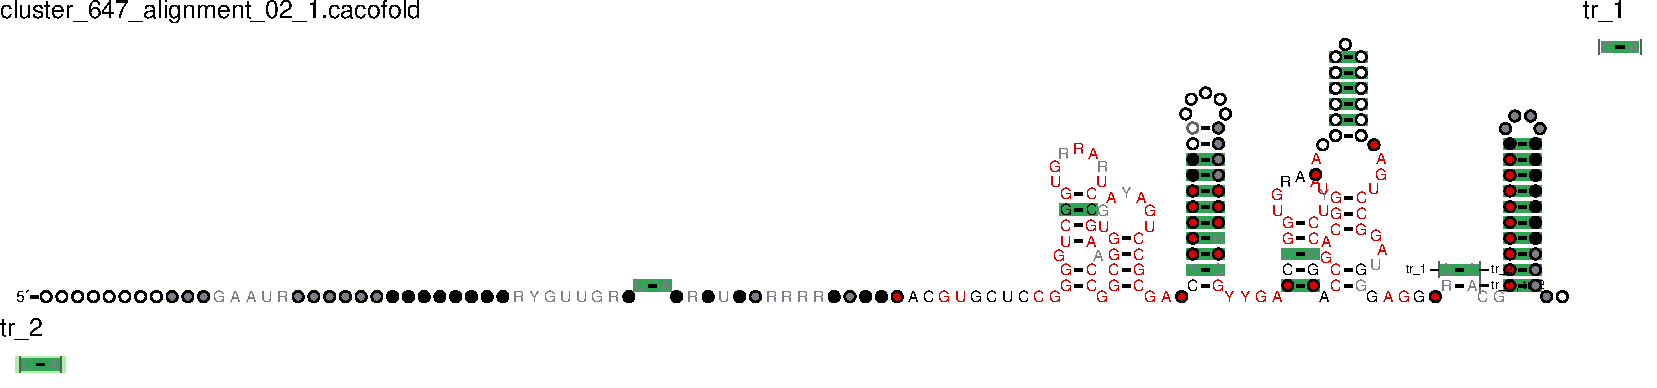
\includegraphics[width=\linewidth]{figures/results/drh-iteritive-expansion-structures/cluster_647_alignment_02_1.cacofold.R2R.sto.pdf}
        \caption{Candidate 647 (F = 73.17)}
        \label{fig:cand647-struct}
    \end{subfigure}

    \vspace{1em}

    \begin{subfigure}[t]{0.48\textwidth}
        \centering
        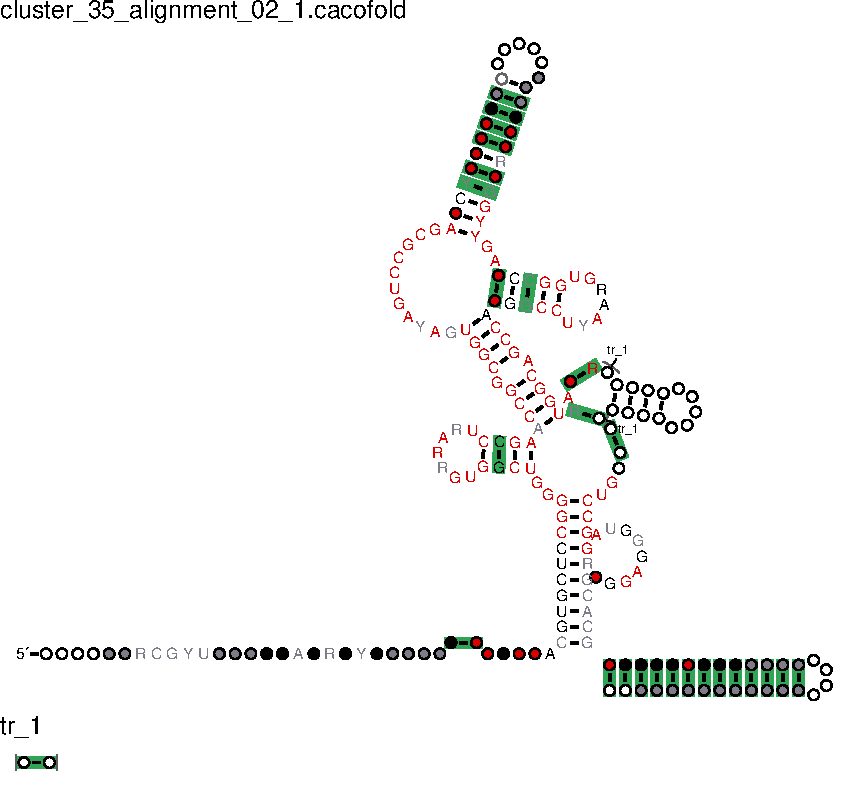
\includegraphics[width=\linewidth]{figures/results/drh-iteritive-expansion-structures/cluster_35_alignment_02_1.cacofold.R2R.sto.pdf}
        \caption{Candidate 35 (F = 62.07)}
        \label{fig:cand35-struct}
    \end{subfigure}
    \hfill
    \begin{subfigure}[t]{0.48\textwidth}
        \centering
        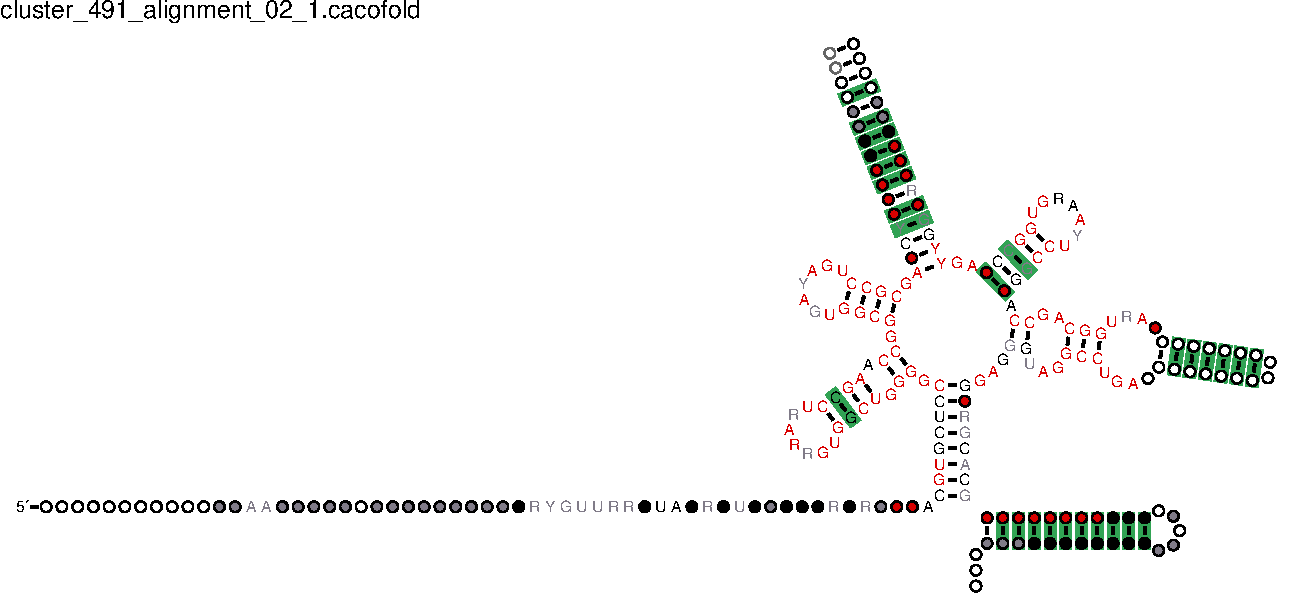
\includegraphics[width=\linewidth]{figures/results/drh-iteritive-expansion-structures/cluster_491_alignment_02_1.cacofold.R2R.sto.pdf}
        \caption{Candidate 491 (F = 60.67)}
        \label{fig:cand491-struct}
    \end{subfigure}

    \vspace{1em}

    \begin{subfigure}[t]{0.48\textwidth}
        \centering
        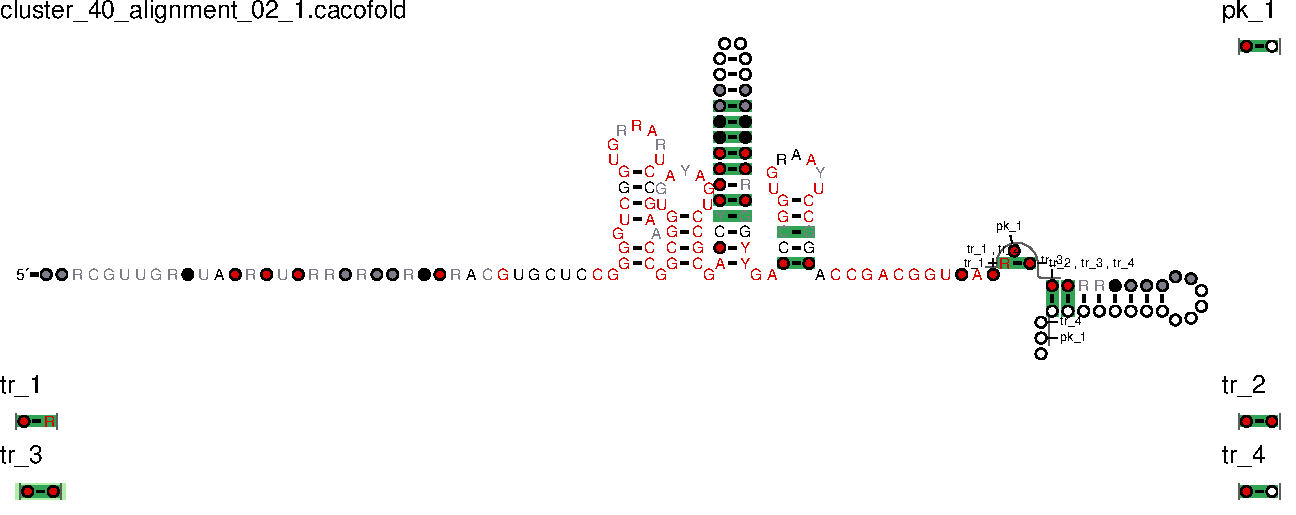
\includegraphics[width=\linewidth]{figures/results/drh-iteritive-expansion-structures/cluster_40_alignment_02_1.cacofold.R2R.sto.pdf}
        \caption{Candidate 40 (F = 56.67)}
        \label{fig:cand40-struct}
    \end{subfigure}

    \caption[Predicted covarying secondary structures of remaining FMN candidates, part 1]{\textbf{Predicted covarying secondary structures of remaining FMN riboswitch candidates (part 1 of 2).} R-scape CaCoFold structures generated from iteratively expanded alignments, ordered by F-score.}
    \label{fig:drh-appendix-structures-1}
\end{figure}

\begin{figure}[p]
    \centering
    \begin{subfigure}[t]{0.48\textwidth}
        \centering
        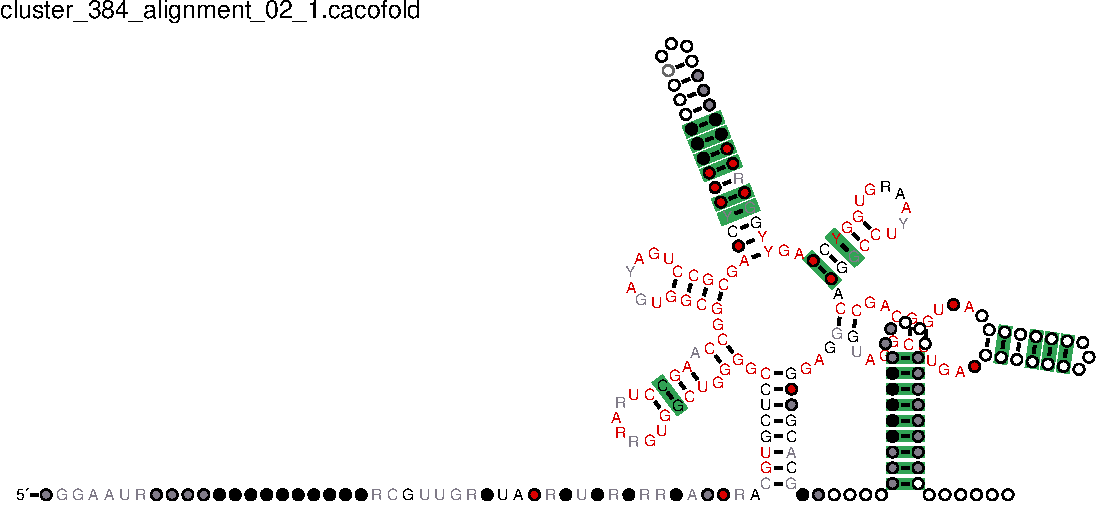
\includegraphics[width=\linewidth]{figures/results/drh-iteritive-expansion-structures/cluster_384_alignment_02_1.cacofold.R2R.sto.pdf}
        \caption{Candidate 384 (F = 55.70)}
        \label{fig:cand384-struct}
    \end{subfigure}
    \hfill
    \begin{subfigure}[t]{0.48\textwidth}
        \centering
        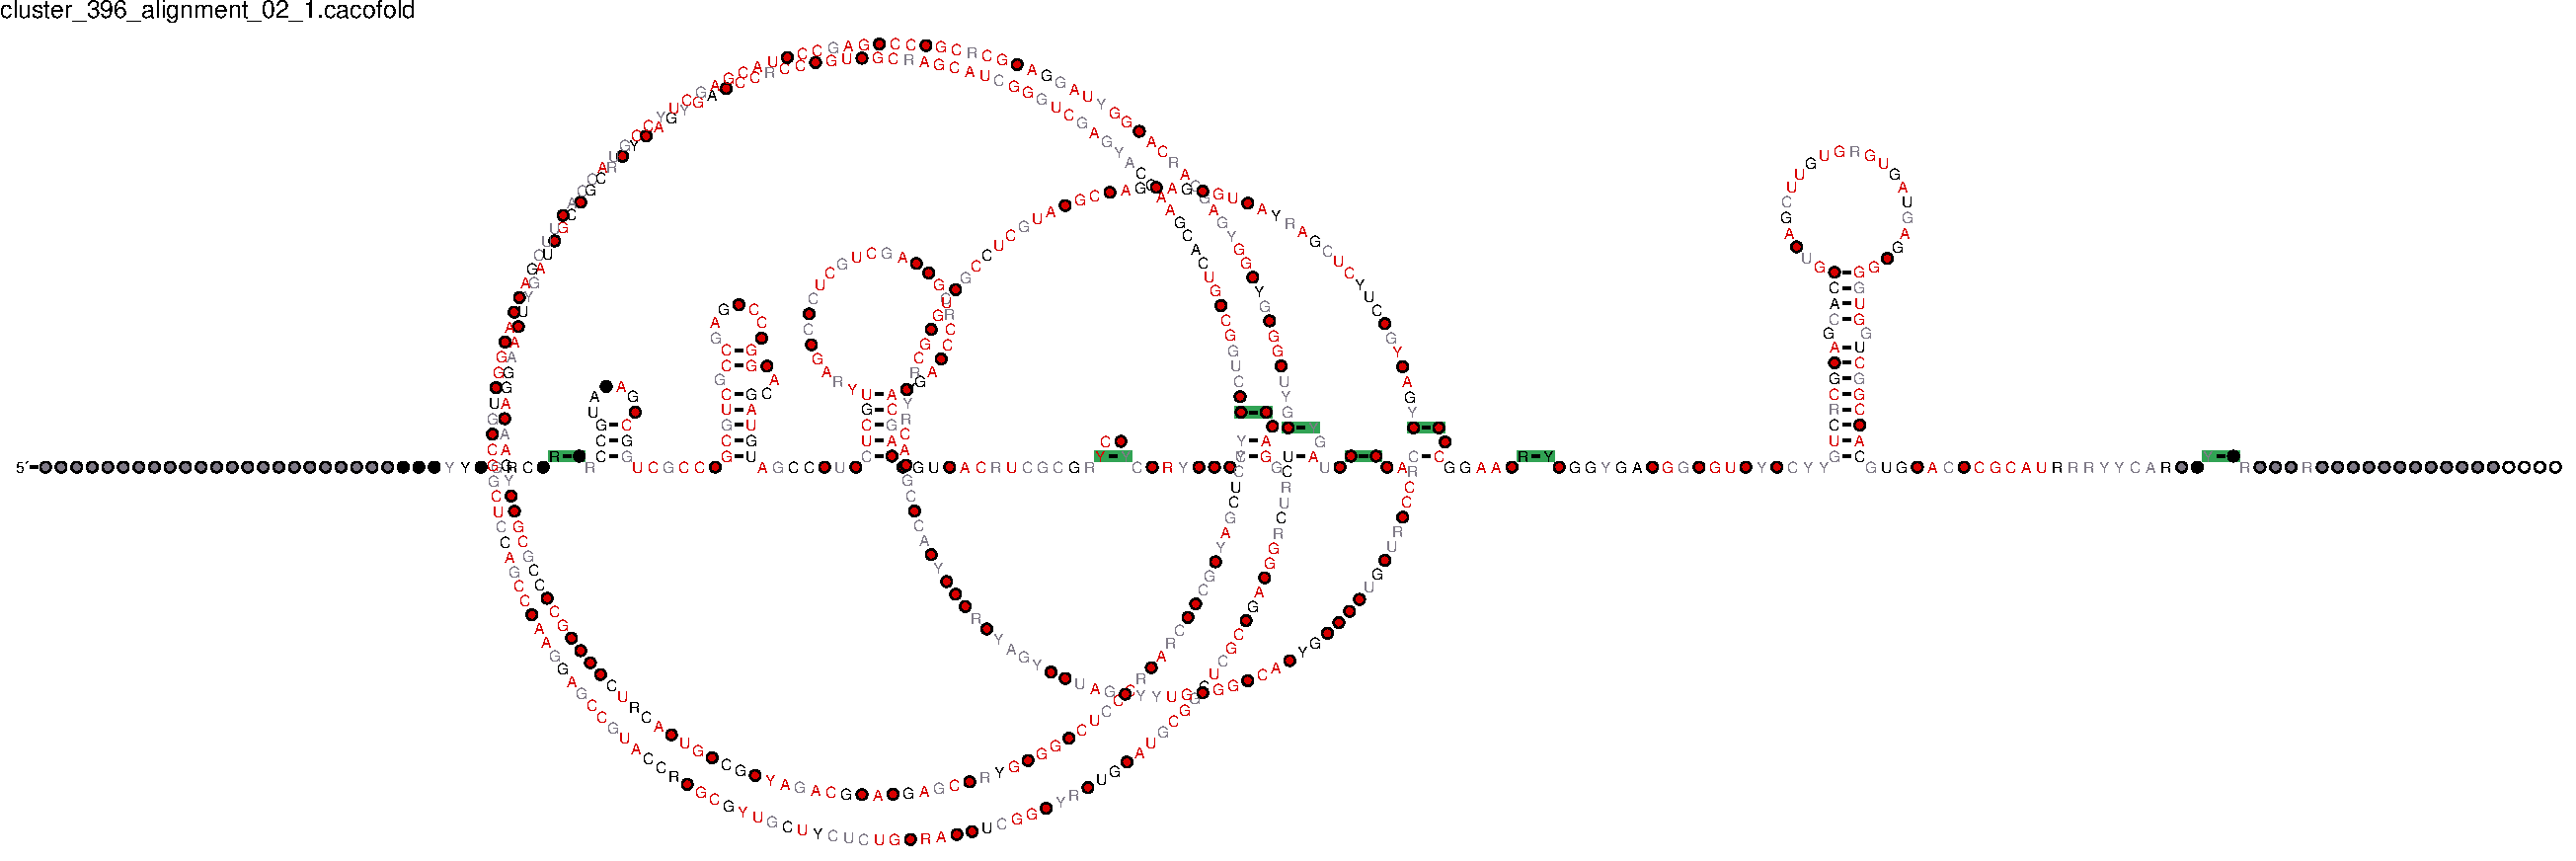
\includegraphics[width=\linewidth]{figures/results/drh-iteritive-expansion-structures/cluster_396_alignment_02_1.cacofold.R2R.sto.pdf}
        \caption{Candidate 396 (F = 34.04)}
        \label{fig:cand396-struct}
    \end{subfigure}

    \vspace{1em}

    \begin{subfigure}[t]{0.48\textwidth}
        \centering
        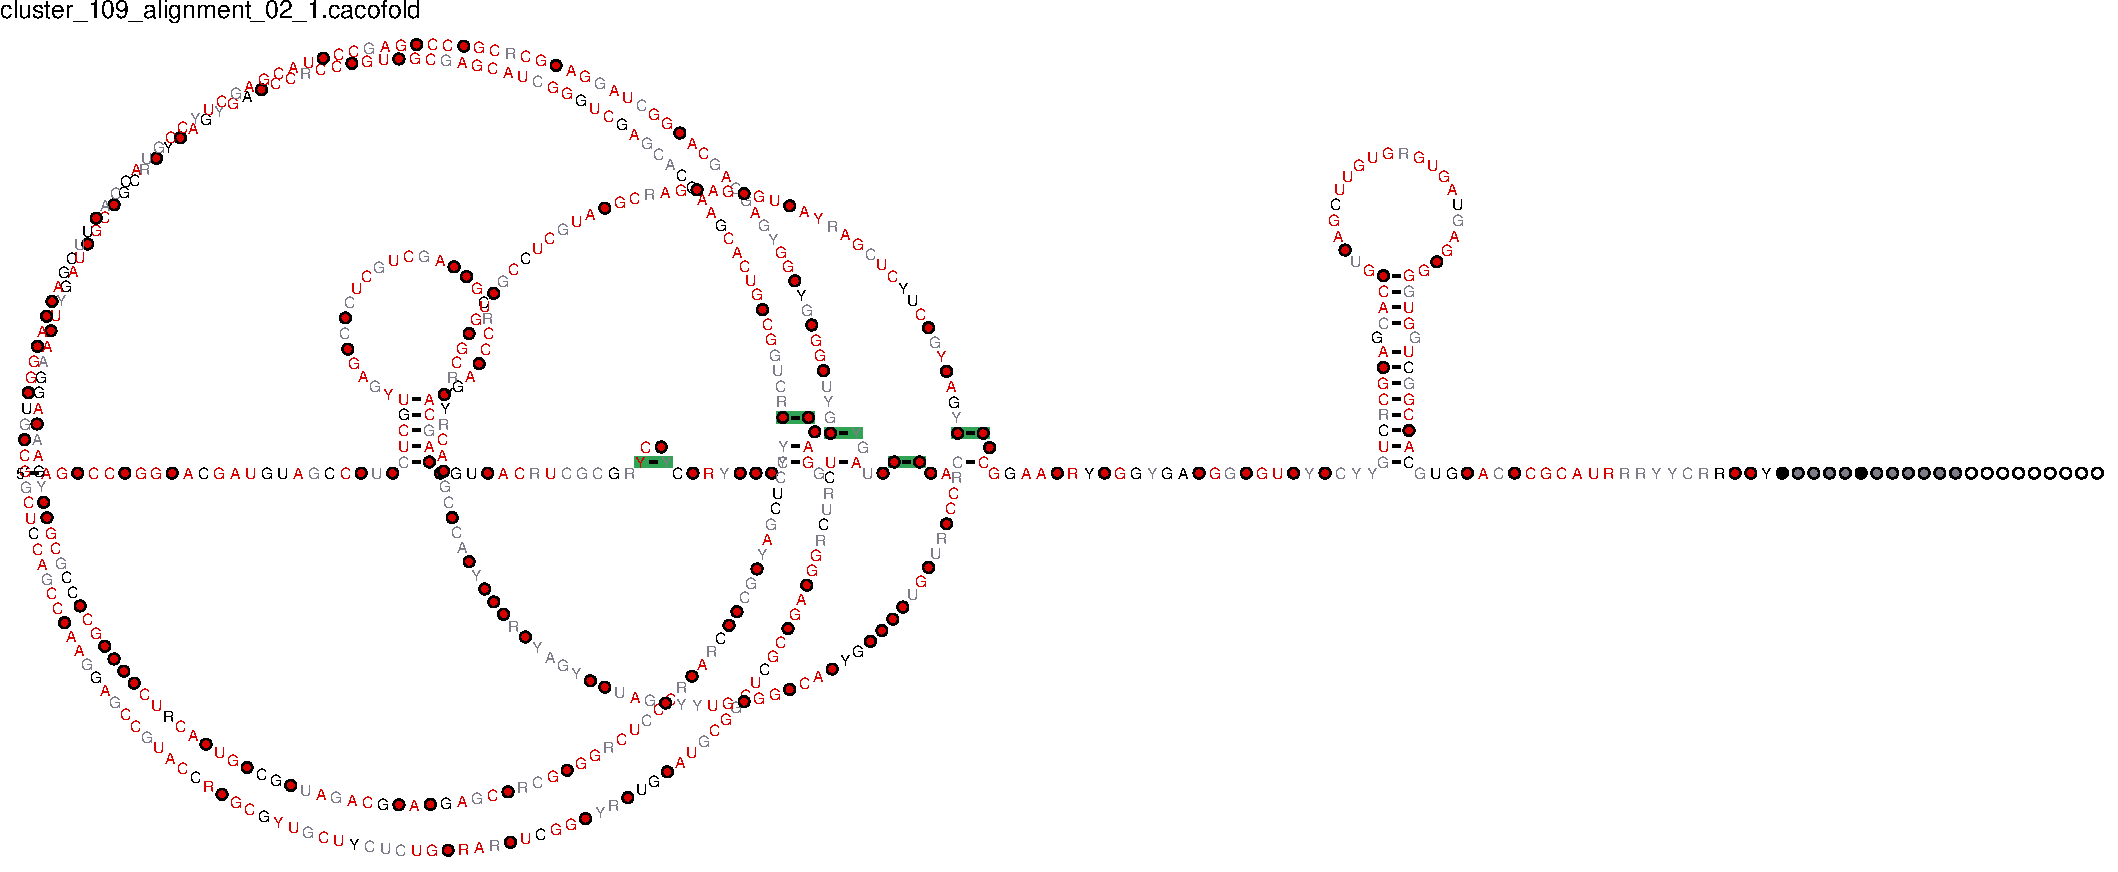
\includegraphics[width=\linewidth]{figures/results/drh-iteritive-expansion-structures/cluster_109_alignment_02_1.cacofold.R2R.sto.pdf}
        \caption{Candidate 109 (F = 32.26)}
        \label{fig:cand109-struct}
    \end{subfigure}
    \hfill
    \begin{subfigure}[t]{0.48\textwidth}
        \centering
        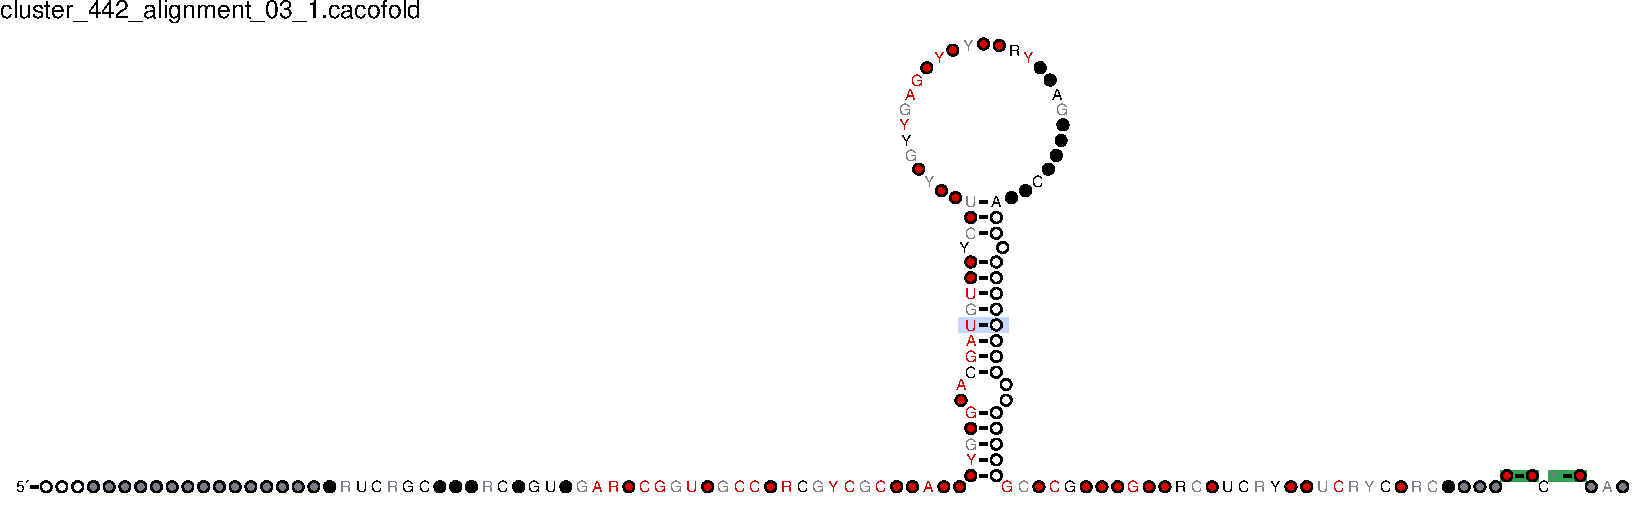
\includegraphics[width=\linewidth]{figures/results/drh-iteritive-expansion-structures/cluster_442_alignment_03_1.cacofold.R2R.sto.pdf}
        \caption{Candidate 442 (F = 20.00)}
        \label{fig:cand442-struct}
    \end{subfigure}

    \caption[Predicted covarying secondary structures of remaining FMN candidates, part 2]{\textbf{Predicted covarying secondary structures of remaining FMN riboswitch candidates (part 2 of 2).} R-scape CaCoFold structures generated from iteratively expanded alignments, ordered by F-score. \ref{fig:cand396-struct} and \ref{fig:cand109-struct} correspond to the two low-identity outlier clusters discussed in the results text.}
    \label{fig:drh-appendix-structures-2}
\end{figure}
\clearpage

\begin{figure}[H]
    \centering
    \begin{subfigure}[t]{0.48\textwidth}
        \centering
        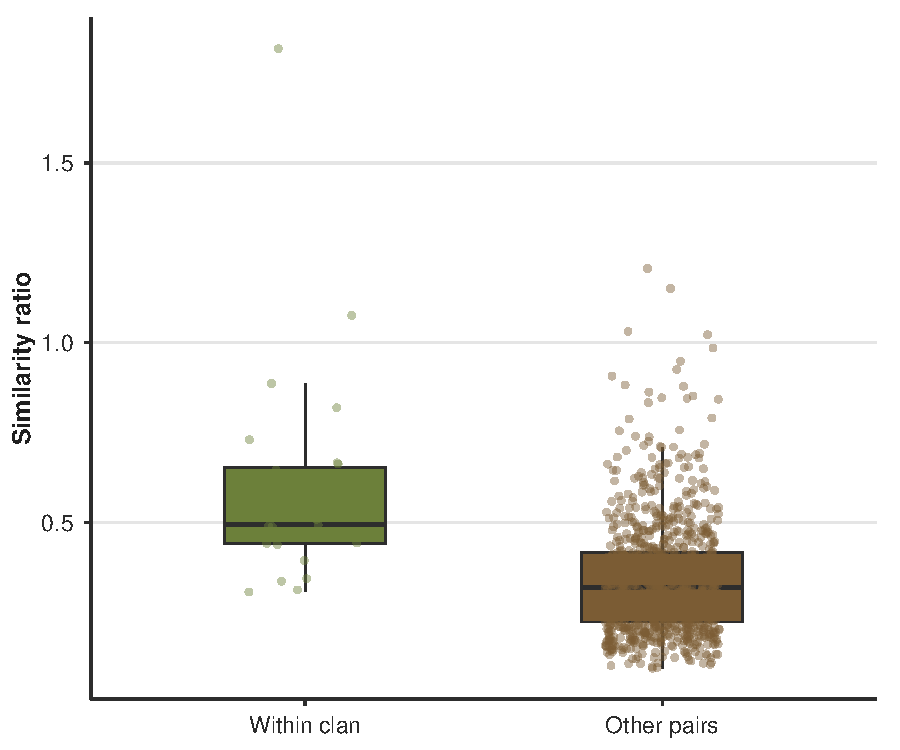
\includegraphics[width=\linewidth]{figures/results/cm-simile/similarity_ratio_boxplot.pdf}
        \caption{Similarity ratio (minmax)}
        \label{fig:similarity-ratio-boxplot}
    \end{subfigure}
    \hfill
    \begin{subfigure}[t]{0.48\textwidth}
        \centering
        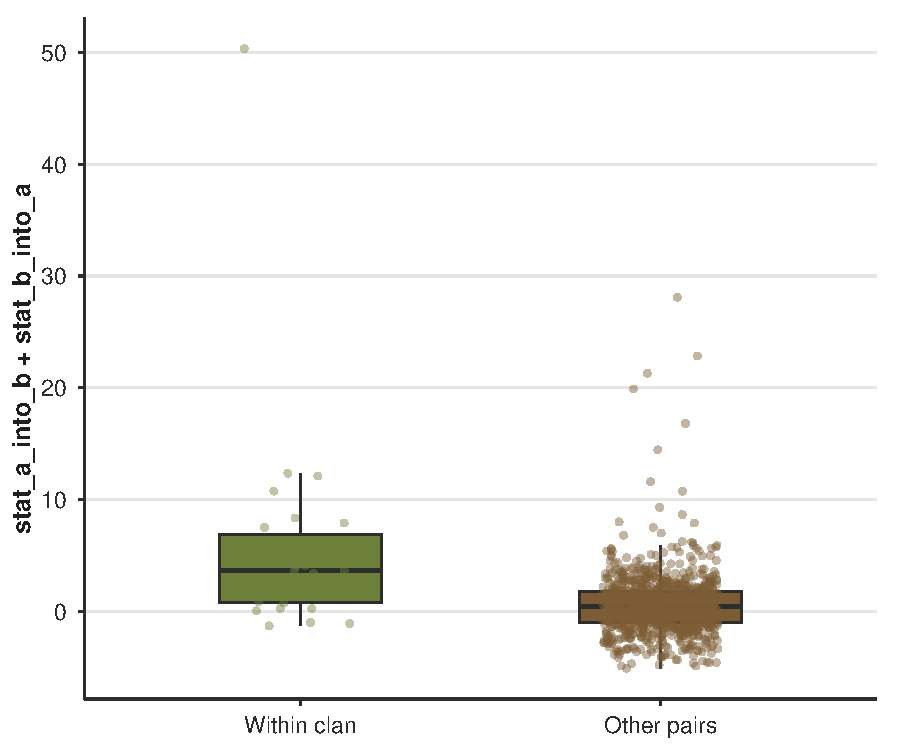
\includegraphics[width=\linewidth]{figures/results/cm-simile/bitscoresumdifference_boxplot.pdf}
        \caption{Bitscore median vs.\ null}
        \label{fig:bitscore-boxplot}
    \end{subfigure}
    \caption[Within- vs.\ between-clan separation for early classification approaches]{\textbf{Within- vs.\ between-clan separation for the two initial classification approaches.} 
    \textbf{(a)}: shows pairwise similarity ratio scores, motivated by common-ancestor theory but lacking a statistical null. 
    \textbf{(b)}: shows median bitscore compared against a dinucleotide-shuffled bootstrap null distribution. 
    Within-clan (\emph{n}~=~27) and other (\emph{n}~=~919) pairs are drawn from annotated Rfam entries.}
    \label{fig:early-classifiers}
\end{figure}

\end{document}
%% All Done!
